\documentclass[a4paper,10pt]{article}
\usepackage[T2A]{fontenc}
\usepackage[utf8]{inputenc}%включаем свою кодировку: koi8-r или utf8 в UNIX, cp1251 в 
\usepackage[english,russian]{babel}%используем русский и английский языки с переносами
\usepackage{amssymb,amsfonts,amsmath,mathtext, esint,cite,enumerate,float,bm,hyperref}
\usepackage{geometry}
\geometry{left=1cm}
\geometry{right=1cm}
\geometry{top=1cm}
\geometry{bottom=2cm}
\usepackage{tikz}
\usepackage{longtable}
\allowdisplaybreaks

\newcommand{\D}{\mathrm{d}}
% Производные
\newcommand{\dsl}[2]{{\partial #1}/{\partial #2}}
\newcommand{\df}[1]{\cfrac{\partial}{\partial #1}}
\newcommand{\dff}[2]{\frac{\partial #1}{\partial #2}}
\newcommand{\dfs}[2]{\frac{\partial^2 #1}{\partial #2^2}}
\newcommand{\dfss}[3]{\frac{\partial^2 #1}{\partial #2\, \partial #3}}
\newcommand{\Df}[1]{\frac{d}{d #1}}
\newcommand{\Dff}[2]{\frac{d #1}{d #2}}
\newcommand{\Dfs}[2]{\frac{d^2 #1}{d #2^2}}
\newcommand{\cDf}[1]{\cfrac{d}{d #1}}
\newcommand{\cDff}[2]{\cfrac{d #1}{d #2}}
\newcommand{\cDfs}[2]{\cfrac{d^2 #1}{d #2^2}}
\newcommand{\dfn}[3]{\frac{\partial^#1 #2}{\partial #3^#1}}
% Векторы
\renewcommand{\vec}[1]{\boldsymbol{#1}}
\newcommand{\ort}[1]{\,\boldsymbol{\mathrm{e}}_#1}
% Векторный анализ
\renewcommand{\div}{\,\mathrm{div}\,}
\newcommand{\rot}{\,\mathrm{rot}\,}
\newcommand{\grad}{\,\mathrm{grad}\,}
\newcommand{\laplas}[4]{\dfs{#1}{#2}+\dfs{#1}{#3}+\dfs{#1}{#4}}
\newcommand{\laplasxyz}[1]{\dfs{#1}{x}+\dfs{#1}{y}+\dfs{#1}{z}}
\newcommand{\rotc}[4]{\dff{#1}{#2} - \dff{#3}{#4}}
\newcommand{\rotcx}[3]{\dff{#1\vphantom{E}_#3}{#2} - \dff{#1\vphantom{E}_#2}{#3}}
% Функции
\renewcommand{\cosh}{\,\mathrm{ch}\,}
\renewcommand{\sinh}{\,\mathrm{sh}\,}
\renewcommand{\tanh}{\,\mathrm{th}\,}
\newcommand{\sign}{\mathrm{\,sgn}\,}
\renewcommand{\Im}{\,\mathrm{Im}\,}
\renewcommand{\Re}{\,\mathrm{Re}\,}
\renewcommand{\det}[4]{#1 #4 - #2 #3}
\renewcommand{\matrix}[4]{\begin{pmatrix}#1 & #2 \\ #3 & #4\end{pmatrix}}
\newcommand{\matrixw}[5]{\begin{#5matrix}#1 & #2 \\ #3 & #4\end{#5matrix}} % #5 = b p s v V
\newcommand{\col}[2]{\begin{pmatrix}#1 & #2\end{pmatrix}}
\newcommand{\colw}[3]{\begin{#3matrix}#1 & #2 \end{#3matrix}} % #3 = b p s v V
\newcommand{\row}[2]{\begin{pmatrix}#1 \\ #2\end{pmatrix}}
\newcommand{\roww}[3]{\begin{#3matrix}#1 \\ #2 \end{#3matrix}} % #3 = b p s v V
\newcommand{\matrixt}[2]{\begin{#1matrix} #2\end{#1matrix}}
\newcommand{\matrixrotr}[7]{\begin{#1matrix} \ort{#2} & \ort{#3} & \ort{#4} \\ \df{#2} & \df{#3} & \df{#4} \\ #5 & #6 & #7 \end{#1matrix}}
\newcommand{\matrixrotd}[4]{\begin{#1matrix} \ort{x} & \ort{y} & \ort{z} \\ \df{x} & \df{y} & \df{z} \\ #2 & #3 & #4 \end{#1matrix}}
\newcommand{\matrixrotdv}[2]{\begin{#1matrix} \ort{x} & \ort{y} & \ort{z} \\ \df{x} & \df{y} & \df{z} \\ #2_x & #2_y & #2_z \end{#1matrix}}
\newcommand{\eps}{\varepsilon}
\renewcommand{\phi}{\varphi}

\newcommand{\shtr}{\mathop{\!\vphantom{E}'}}
\newcommand{\ind}[1]{\mathop{\!\vphantom{E}_{#1}}}

\setlength{\parindent}{0cm}
\begin{document}
\tableofcontents
\clearpage

\documentclass[a4paper,10pt]{article} %размер бумаги устанавливаем А4, шрифт 12пунктов
\usepackage[T2A]{fontenc}
\usepackage[utf8]{inputenc}%включаем свою кодировку: koi8-r или utf8 в UNIX, cp1251 в 
\usepackage[english,russian]{babel}
\usepackage{amssymb,amsfonts,amsmath,mathtext,cite,enumerate,float}
\usepackage{hyperref}
\renewcommand{\rmdefault}{ftm}

\usepackage{geometry}
\geometry{left=1cm}
\geometry{right=1cm}
\geometry{top=1cm}
\geometry{bottom=1cm}

\begin{document}
	
	Вспомним что:
	$$
		\sin x = A x \prod\limits_{n = 1}^{\infty} \left(1 - \frac{x^2}{\pi^2 n^2}\right) =
		A x \left[
		1 -
		\frac{x^2}{\pi^2} \left(1 + \frac{1}{2^2} + \frac{1}{3^2} + \ldots \right) +
		\frac{x^4}{\pi^4} \alpha_4 + 
		\frac{x^6}{\pi^6} \alpha_6 + \ldots
		\right]
	$$
	Теперь:
	$$
		\sin x = x - \frac{x^3}{6} + \frac{x^5}{120} - \ldots
	$$
	и финт ушами:
	$$
		\left(1 + \frac{1}{2^2} + \frac{1}{3^2} + \ldots \right)^2 = 
		1 + \frac{1}{2^4} + \frac{1}{3^4} + \ldots + 2 \alpha_4
	$$
	Ба-бах:
	$$
		1 + \frac{1}{2^4} + \frac{1}{3^4} + \ldots = \frac{\pi^4}{36} - 2 \frac{\pi^4}{120} = \frac{\pi^4}{90}
	$$

\end{document}

\section{Сферические координаты}

Связь декартовых $(x, y, z)$ и сферических координат $(r, \theta, \alpha)$ даётся выражениями:
\[
	\begin{aligned}
		& x = r \sin \theta \cos \alpha \\
		& y = r \sin \theta \sin \alpha \\
		& z = r \cos \theta 
	\end{aligned}
\]
Орты сферической системы координат найдём из соотношений:
\[
	\begin{aligned}
	& \left|\frac{\partial \vec{r}}{\partial r}\right| \vec{e}_r = \frac{\partial \vec{r}}{\partial r} =  \sin \theta \cos \alpha\, \vec{e}_x + \sin \theta \sin \alpha\, \vec{e}_y + \cos \theta\, \vec{e}_z \\
	& \left|\frac{\partial \vec{r}}{\partial \theta}\right| \vec{e}_\theta = \frac{\partial \vec{r}}{\partial \theta} =  r \cos \theta \cos \alpha\, \vec{e}_x + r \cos \theta \sin \alpha\, \vec{e}_y - r \sin \theta\, \vec{e}_z \\
	& \left|\frac{\partial \vec{r}}{\partial \alpha}\right| \vec{e}_\alpha = \frac{\partial \vec{r}}{\partial \alpha} = - r \sin \theta \sin \alpha\, \vec{e}_x + r \sin \theta \cos \alpha\, \vec{e}_y
	\end{aligned}
\]
Коэффициенты Ламе:
\[
	\begin{aligned}
		& H_r =  \left|\frac{\partial \vec{r}}{\partial r}\right| = 1 \\
		& H_\theta = \left|\frac{\partial \vec{r}}{\partial \theta}\right| = r \\
		& H_\alpha = \left|\frac{\partial \vec{r}}{\partial \alpha}\right| = r \sin \theta
	\end{aligned}
\]
Орты
\[
	\begin{aligned}
	& \vec{e}_r = \sin \theta \cos \alpha\, \vec{e}_x + \sin \theta \sin \alpha\, \vec{e}_y + \cos \theta\, \vec{e}_z \\
	& \vec{e}_\theta = \cos \theta \cos \alpha\, \vec{e}_x + \cos \theta \sin \alpha\, \vec{e}_y - \sin \theta\, \vec{e}_z \\
	& \vec{e}_\alpha = -\sin \alpha\, \vec{e}_x + \cos \alpha\, \vec{e}_y
	\end{aligned}
\]
Орты декартовой системы, выраженные через орты сферической системы:
\[
	\begin{aligned}
	& \vec{e}_x = \sin \theta \cos \alpha\, \vec{e}_r + \cos \theta \cos \alpha\, \vec{e}_\theta -\sin \alpha\,  \vec{e}_\alpha \\
	& \vec{e}_y = \sin \theta \sin \alpha\, \vec{e}_r + \cos \theta \sin \alpha\, \vec{e}_\theta + \cos \alpha\, \vec{e}_\alpha \\
	& \vec{e}_z = \cos \theta\,\vec{e}_r - \sin \theta\, \vec{e}_\theta
	\end{aligned}
\]
Немного о производных от ортов (для вывода нужно помнить, что орты декартовой системы образуют базис, не зависящий от его положения, в то время как орты сферической системы образуют базис, который меняется от точки к точке):
\[
	\begin{aligned}
	& \frac{\partial \vec{e}_r}{\partial r} = 0 \\
	& \frac{\partial \vec{e}_r}{\partial \theta} = \vec{e}_\theta \\
	& \frac{\partial \vec{e}_r}{\partial \alpha} = \sin \theta\, \vec{e}_\alpha
	\end{aligned}
	\quad
	\begin{aligned}
	& \frac{\partial \vec{e}_\theta}{\partial r} = 0 \\
	& \frac{\partial \vec{e}_\theta}{\partial \theta} = -\vec{e}_r \\
	& \frac{\partial \vec{e}_\theta}{\partial \alpha} = \cos \theta\, \vec{e}_\alpha
	\end{aligned}
	\quad
	\begin{aligned}
	& \frac{\partial \vec{e}_\alpha}{\partial r} = 0 \\
	& \frac{\partial \vec{e}_\alpha}{\partial \theta} = 0 \\
	& \frac{\partial \vec{e}_\alpha}{\partial \alpha} = -\sin\theta \, \vec{e}_r -\cos \theta\, \vec{e}_\theta
	\end{aligned}
\]

\section{Волновые функции в $p$ и $x$ представлениях}

Для описания квантовых процессов вводят волновые функции, которые являются суперпозициями волн д'Бройля. Для одной частицы:
\[
	\psi(\vec{r}, t) = A \int C_(\vec{p}, t) \exp \left(\frac{i}{\hbar} \vec{p} \cdot \vec{r}\right) d^3p
\]
\[
	C(\vec{p}, t) = B \int \psi(\vec{r}, t) \exp \left(-\frac{i}{\hbar} \vec{p} \cdot \vec{r}\right) d^3r
\]
$\psi(\vec{r}, t)$ -- волновая функция в $x$ представлении. $C(\vec{p}, t)$ -- волновая функция в $p$ представлении. $A$ и $B$ -- действительные числа, которые можно найти из условия нормировки. Нормировка:
\[
	\int \psi^*(\vec{r}, t) \psi(\vec{r}, t) d^3r = \int C^*(\vec{p}, t) C(\vec{p}, t) d^3p = 1
\]
\[
	\begin{gathered}
		A^2\iint C^*(\vec{p'}, t) C(\vec{p}, t) \exp \left(\frac{i}{\hbar} (\vec{p'} - \vec{p}) \cdot \vec{r}\right) d^3p\, d^3p'\, d^3r 
		= \\
		=
		A^2\int C^*(\vec{p'}, t) C(\vec{p}, t) (2\pi \hbar)^3 \delta(\vec{p'} - \vec{p}) d^3p\, d^3p'
		= \\
		=
		A^2 (2\pi \hbar)^3 \int C^*(\vec{p}, t) C(\vec{p}, t) d^3p = A^2 (2\pi \hbar)^3 = 1
	\end{gathered}
\]
\[
	\begin{gathered}
		B^2\iint \psi^*(\vec{r'}, t) \psi(\vec{r}, t) \exp \left(\frac{i}{\hbar} \vec{p} \cdot (\vec{r'} - \vec{r})\right) d^3p \, d^3r \, d^3r'
		= \\
		=
		B^2 (2\pi\hbar)^3 \iint \psi^*(\vec{r'}, t) \psi(\vec{r}, t) \delta(\vec{r'} - \vec{r}) d^3r \, d^3r' = B^2 (2\pi\hbar)^3 \iint \psi^*(\vec{r}, t) \psi(\vec{r}, t) d^3r 
		= \\
		=
		B^2 (2\pi\hbar)^3 = 1
	\end{gathered}
\]
\[
	A = B =\frac{1}{(2\pi\hbar)^{3/2}}
\]
Обратимость непосредственно следует из обратимости преобразования Фурье.

\section{Оператор импульса в $x$ представлении}
Оператор импульса в $p$ представлении, просто вектор $\vec{p}$. 
По определению оператор импульса $\hat{\vec{p}}$ в $x$ представлении:
\[
	\langle \vec{p} \,\rangle = \int \psi^*(\vec{r}, t) \hat{\vec{p}} \psi(\vec{r}, t) d^3r
\]
Средний импульс:
\[
	\begin{gathered}
	\langle \vec{p} \,\rangle = 
	\int C^*(\vec{p}, t) \vec{p} C(\vec{p}, t) d^3p = \\ =
	\frac{1}{(2\pi\hbar)^{3}} \iiint \vec{p} \psi^*(\vec{r'}, t) \psi(\vec{r}, t) \exp \left(\frac{i}{\hbar} \vec{p} \cdot (\vec{r'} - \vec{r})\right) d^3r'\, d^3r\, d^3p = \\ =
	\frac{1}{(2\pi\hbar)^{3}} \iint \psi^*(\vec{r'}, t) \psi(\vec{r}, t) \frac{\hbar}{i}\frac{\partial}{\partial \vec{r'}}\int\exp \left(\frac{i}{\hbar} \vec{p} \cdot (\vec{r'} - \vec{r})\right) d^3p\, d^3r'\, d^3r = \\ =
	\iint \psi^*(\vec{r'}, t) \psi(\vec{r}, t) \frac{\hbar}{i} \frac{\partial}{\partial \vec{r'}} \delta(\vec{r'} - \vec{r}) d^3r'\, d^3r = \\ =
	[\text{интегрируем по частям и учитываем, что $\psi = 0$ на $\infty$}] =
	\end{gathered}
\]
\[
	\begin{gathered}
	= - \frac{\hbar}{i} \iint \delta(\vec{r'} - \vec{r}) \frac{\partial}{\partial \vec{r'}} \psi^*(\vec{r'}, t) \psi(\vec{r}, t) d^3r'\, d^3r = \\ =
	- \frac{\hbar}{i} \int \psi(\vec{r}, t) \frac{\partial}{\partial \vec{r}} \psi^*(\vec{r}, t) d^3r = \\ =
	[\text{ещё одно интегрирование по частям}] = \\ =
	\frac{\hbar}{i} \int \psi^*(\vec{r}, t) \frac{\partial}{\partial \vec{r}} \psi(\vec{r}, t) d^3r
	\end{gathered}
\]
\[
	\hat{\vec{p}} = \frac{\hbar}{i} \frac{\partial}{\partial \vec{r}} = - i \hbar \frac{\partial}{\partial \vec{r}}
\]

\section{Оператор координаты в $p$ представлении}
Оператор координаты в $x$ представлении $\vec{r}$. В $p$ представлении по определению:
\[
	\langle \vec{r}\,\rangle = \int C^*(\vec{p}, t) \hat{\vec{r}} C(\vec{p}, t) d^3p	
\]
Итак:
\[
	\begin{gathered}
	\langle \vec{r}\,\rangle = \int \psi^*(\vec{r}, t) \vec{r} \psi(\vec{r}, t) d^3 r = \\ =
	\frac{1}{(2\pi\hbar)^{3}} \iiint C^*(\vec{p'}, t) C(\vec{p}, t) \vec{r} 
	\exp 
	\left(
		-\frac{i}{\hbar}
			(\vec{p'} - \vec{p})\cdot \vec{r}
	\right) d^3r\,d^3p\,d^3p' =
	\\ =
	\frac{1}{(2\pi\hbar)^{3}} \iint C^*(\vec{p'}, t) C(\vec{p}, t)
	\frac{\hbar}{i}
	\frac{\partial}{\partial \vec{p}}
	\int
	\exp 
	\left(
		\frac{i}{\hbar}
		(\vec{p} - \vec{p'})\cdot \vec{r}
	\right) d^3r\,d^3p\,d^3p' = 
	\\ =
	\frac{\hbar}{i}\iint C^*(\vec{p'}, t) C(\vec{p}, t)
	\frac{\partial}{\partial \vec{p}}
	\delta(\vec{p} - \vec{p'}) d^3p\, d^3p'
	= \\ =
	[\text{интегрируем по частям и учитываем, что $C = 0$ на $\infty$}] = \\ =
	-\frac{\hbar}{i}
	\iint 
	C^*(\vec{p}, t)
	\frac{\partial}{\partial \vec{p}}
	C(\vec{p}, t)
	d^3p
	\end{gathered}
\]
В результате:
\[
	\hat{\vec{r}} = 
	-\frac{\hbar}{i} \frac{\partial}{\partial \vec{p}} =
	i\hbar \frac{\partial}{\partial \vec{p}} 
\]
Уравнение Шрёдингера сохраняет свою форму:
\[
	\sum_{i=1}^N\frac{p_i^2}{2m_i} C + \hat{U}\left(i \hbar \frac{\partial}{\partial p_1}, \ldots, i \hbar \frac{\partial}{\partial p_N}\right) C = i\hbar \frac{\partial C}{\partial t}
\]
\section{Определение и некоторые свойства функций Эйри}

Функциями Эйри называют:
\[
	\mathrm{Ai\,}(x) = \frac{1}{\pi} \int\limits_0^\infty \cos \left( \frac{t^3}{3} + xt\right) dt
\]
\[
	\mathrm{Bi\,}(x) = \frac{1}{\pi} \int\limits_0^\infty \left[e^{-\frac{1}{3}t^3 - xt} + \sin \left( \frac{t^3}{3} + xt\right)\right] dt
\]
Асимптотика (можно найти, проинтегрировав методом перевала в комплексной плоскости):
\[
	\mathrm{Ai\,}(x) \underset{x \to \infty}{\approx} \frac{1}{2\sqrt{\pi} x^{1/4}} \exp \left( -\frac{2}{3} x^{3/2}\right)
\]
\[
	\mathrm{Bi\,}(x) \underset{x \to \infty}{\approx} \frac{1}{\sqrt{\pi} x^{1/4}} \exp \left( \frac{2}{3} x^{3/2}\right)
\]
\[
	\mathrm{Ai\,}(x) \underset{x \to -\infty}{\approx} \frac{1}{\sqrt{\pi} x^{1/4}} \sin \left( \frac{2}{3} |x|^{3/2} + \frac{\pi}{4}\right)
\]
\[
	\mathrm{Bi\,}(x) \underset{x \to -\infty}{\approx} \frac{1}{\sqrt{\pi} x^{1/4}} \cos \left( \frac{2}{3} |x|^{3/2}+ \frac{\pi}{4}\right)
\]
Интеграл (легко находится с использованием дельта функции)
\[
	\int\limits_{-\infty}^{\infty} \mathrm{Ai\,}(x)\, dx = 1
\]
Функции Эйри удовлетворяют уравнению Эйри:
\[
	u'' - xu = 0
\]
Рассмотрим интеграл:
\[
	\int\limits_{a}^{\infty}\mathrm{\,Ai\,}'(x) \mathrm{\,Ai\,}''(x) dx= 
	\int\limits_{a}^{\infty} x \mathrm{\,Ai\,}'(x) \mathrm{\,Ai\,}(x) dx
\]
\[
	\Rightarrow \frac{\left[\mathrm{\,Ai\,}'(x) \right]^2}{2} \Bigg|_{a}^{\infty} =
	x \frac{\left[\mathrm{\,Ai\,}(x) \right]^2}{2} \Bigg|_{a}^{\infty} - 
	\int\limits_{a}^{\infty} \frac{\left[\mathrm{\,Ai\,}(x) \right]^2}{2} dx
\]
Откуда следует весьма важный интеграл:
\[
	\int\limits_{a}^{\infty} \left[\mathrm{\,Ai\,}(x) \right]^2 dx =
	\left[\mathrm{\,Ai\,}'(a) \right]^2  - a \left[\mathrm{\,Ai\,}(a) \right]^2
\]

\section{Решение линейных уравнений}

Поставим следующую задачу:
\[
	L\left[y\right] = \frac{\partial y}{\partial t} 
\]
\[
	y(x, t)\Big|_{t = 0} = y(x, 0) 
\]
$L$ -- произвольный линейный оператор.
Пусть собственные значения $Y(x, \lambda)$ удовлетворяет уравнению:
\[
	L\left[Y\right] = \lambda Y
\]
и если спектр $\lambda$ сплошной, существует функция $Y^{-1}(x, \lambda')$, такая что:
\[
	\int\limits_{-\infty}^{\infty} Y^{-1}(x, \lambda') Y(x, \lambda) dx = \delta(\lambda - \lambda')
\]
Будем искать $y$ в виде:
\[
	y = \int\limits_{-\infty}^{\infty} A(\lambda) e^{\lambda t} Y(x, \lambda)\, d\lambda
\]
Простой подстановкой можно проверить, что это выражение в самом деле является решением уравнения. $A(\lambda)$ определим из начальных условий:
\[
	y(x, 0) = \int\limits_{-\infty}^{\infty} A(\lambda) Y(x, \lambda)\, d\lambda
\]
\[
	A(\lambda) = \int\limits_{-\infty}^{\infty} y(x, 0) Y^{-1}(x, \lambda)\, dx
\]
Подставляем в решение и получаем:
\[
	y(x, t) = \int\limits_{-\infty}^{\infty} y(x', 0) \int\limits_{-\infty}^{\infty} e^{\lambda t}Y^{-1}(x', \lambda) Y(x, \lambda)\, d\lambda\, dx'
\]

\section{Решение линейных уравнений в случае дискретного спектра}

В случае дискретного спектра у нас есть система функций:
\[
	Y_1(x), Y_2(x), \ldots, Y_n(x), \ldots
\]
и соответствующая ей последовательность чисел:
\[
	\lambda_1, \lambda_2, \ldots
\]
Если удалось построить дополнительную систему функций
\[
	Y_1^{-1}(x), Y_2^{-1}(x), \ldots, Y_n^{-1}(x), \ldots
\]
такую что
\[
	\int\limits_{-\infty}^{\infty} Y_k^{-1}(x) Y_n(x) dx = \delta_{kn}
\]
То решение уравнения можно найти в виде:
\[
	y = \sum_{k=1}^{\infty} A_k e^{\lambda_k t} Y_k(x)
\]
\[
	A_k = \int\limits_{-\infty}^{\infty} Y_k^{-1}(x) y(x, 0) dx
\]
Получаем окончательно решение:
\[
	y(x, t) = \int\limits_{-\infty}^{\infty} y(x', 0) \sum_{k=1}^{\infty} e^{\lambda_k t} Y_k^{-1}(x') Y_k(x) dx'
\]
\section{Частица в однородном силовом поле}

Пусть сила, действующая на частицу, равна $F$ по модулю и направлена вдоль оси $z$ в обратном направлении. Гамильтониан в классическом случае:
\[
	\hat{H} = \frac{\hat{p}_z^2}{2m} + F \hat{z} 
\]
Уравнение Шрёдингера:
\[
	\frac{p_z^2}{2m} C(p_z, t) + i \hbar F \frac{\partial C(p_z, t)}{\partial p_z} = i\hbar \frac{\partial C(p_z, t)}{\partial t}
\]
Вместо $\lambda$ будет выступать $-iE/\hbar$. Для $Y$ получаем уравнение
\[
	\frac{p_z^2}{2m} Y + i \hbar F \frac{\partial Y}{\partial p_z} = E Y
\]
Будем искать $Y$ в форме $\exp f(p_z)$:
\[
	i \hbar F \frac{\partial f(p_z)}{\partial p_z} = E - \frac{p_z^2}{2m}
\]
\[
	f(p_z) = - i \frac{E}{\hbar F} p_z + i \frac{1}{6 m \hbar F} p_z^3 + const
\]
Константа уйдёт в нормировочный множитель. 
\[
	Y(p_z, E) = A \exp \left(-\frac{i}{\hbar} \left( \frac{E}{F} p_z - \frac{1}{6 m F} p_z^3 \right) \right)
\]
\[
	Y^{-1}(p_z, E) = B \exp \left(\frac{i}{\hbar} \left( \frac{E}{F} p_z - \frac{1}{6 m F} p_z^3 \right) \right)
\]
\[
	AB \int\limits_{-\infty}^{\infty} \exp \left(\frac{i p_z}{\hbar F} (E' - E) \right) dp_z = 
	2\pi AB\hbar F\, \delta(E' - E) = \delta(E' - E)
\]
Откуда можно в качестве $A$ и $B$ можно взять константы:
\[
	A = B = \frac{1}{\sqrt{2\pi \hbar F}}
\]
\[
	\begin{gathered}
		C(p_z, t) = \int\limits_{-\infty}^{\infty} C(p_z, 0) \int\limits_{-\infty}^{\infty} AB
		\exp \left(-\frac{i}{\hbar} \left( E \left(\frac{p_z - p_z'}{F} + t\right) - \frac{1}{6 m F} (p_z^3 - p_z'^3) \right)
		\right)\, dE\, dp_z' = \\
		=
		\int\limits_{-\infty}^{\infty} C(p_z', 0) \delta(p_z - p_z' + F t) 
		\exp \left(\frac{i}{6 m \hbar F} (p_z^3 - p_z'^3) \right)
		\, dp_z' = \\
		=
		C(p_z + F t, 0) \exp \left(\frac{i(-3 p_z^2 F t - 3 p_z F^2 t^2 - F^3 t^3)}{6 m \hbar F} \right) = \\
		=
		C(p_z + F t, 0) \exp \left(-\frac{i}{\hbar} \left(\frac{p_z^2}{2m} t + \frac{p_z F t^2}{2 m} + \frac{F^2 t^3}{6 m}\right) \right)
	\end{gathered}
\]
Чтобы получить дискретный спектр нужно ввести дополнительные условия. Чаще всего таким условием выступает поверхность, за пределы которой частица не может попасть. В качестве такой поверхности может выступать поверхность Земли для поля тяжести, обкладка конденсатора.

\section{Гауссовский волновой пакет в однородном поле}

Пусть
\[
	\psi(z, 0) = \frac{1}{\sqrt[4]{2\pi \sigma^2}} \exp \left( -\frac{(z - z_0)^2}{4\sigma^2}\right)
\]
\[
	\begin{gathered}
		C(p_z, 0) = \frac{1}{\sqrt[4]{2\pi \sigma^2}}\frac{1}{(2\pi\hbar)^{1/2}} \int\limits_{-\infty}^{\infty} \exp \left(-\frac{(z - z_0)^2}{4\sigma^2} - \frac{i}{\hbar} p_z z  \right) dz = \\
		=
		\frac{1}{\sqrt[4]{2\pi \sigma^2}}\frac{1}{(2\pi\hbar)^{1/2}} \exp\left(-\frac{i}{\hbar}p_z z_0\right)\int\limits_{-\infty}^{\infty} \exp \left(-\frac{(z - z_0)^2}{4\sigma^2} - \frac{i}{\hbar} p_z (z - z_0)  \right) dz = \\
		=
		\frac{1}{\sqrt[4]{2\pi \sigma^2}}\frac{1}{(2\pi\hbar)^{1/2}} \exp\left(-\frac{i}{\hbar}p_z z_0\right)
		\int\limits_{-\infty}^{\infty} \exp \left(-\frac{(z - z_0)^2}{4\sigma^2} - 2 \frac{i}{\hbar} \sigma p_z \frac{(z - z_0)}{2 \sigma}  \right) dz = \\
		=
		\frac{1}{\sqrt[4]{2\pi \sigma^2}}\frac{1}{(2\pi\hbar)^{1/2}} \exp\left(-\frac{i}{\hbar}p_z z_0\right)
		\int\limits_{-\infty}^{\infty} \exp \left(-\left(\frac{(z - z_0)}{2 \sigma} + \frac{i}{\hbar} \sigma p_z \right)^2 - \frac{\sigma^2 p_z^2}{\hbar^2}  \right) dz = \\
		=
		\frac{2\sqrt[4]{2\pi \sigma^2}}{(2\pi\hbar)^{1/2}} \exp\left(-\frac{i}{\hbar}p_z z_0 - \frac{\sigma^2 p_z^2}{\hbar^2} \right) = \\
		=
		\sqrt[4]{\frac{2\sigma^2}{\pi \hbar^2}} \exp\left(-\frac{i}{\hbar}p_z z_0 - \frac{\sigma^2 p_z^2}{\hbar^2} \right)
	\end{gathered}
\]
\[
	\begin{gathered}
		\langle z \rangle =
		\sqrt{\frac{2\sigma^2}{\pi \hbar^2}} 
		\int\limits_{-\infty}^{\infty} \left(z_0 - \frac{2i\hbar \sigma^2}{\hbar^2} (p_z + Ft) + \frac{p_z}{m} t +  \frac{F t^2}{2m}\right) 
		\exp\left( - \frac{2\sigma^2 (p_z + Ft)^2}{\hbar^2} \right) dp_z = \\
		=
		\sqrt{\frac{2\sigma^2}{\pi \hbar^2}} 
		\int\limits_{-\infty}^{\infty} \left(z_0 - \frac{2i\hbar \sigma^2}{\hbar^2} (p_z + Ft) + \frac{p_z + F t}{m} t -  \frac{F t^2}{2m}\right) 
		\exp\left( - \frac{2\sigma^2 (p_z + Ft)^2}{\hbar^2} \right) dp_z = \\
		=
		z_0 - \frac{F t^2}{2m}	
	\end{gathered}
\]
\[
	\begin{gathered}
		\langle z^2 \rangle =
		\sqrt{\frac{2\sigma^2}{\pi \hbar^2}} 
		\int\limits_{-\infty}^{\infty} \left(z_0 - \frac{F t^2}{2m} + \left(\frac{t}{m}- 2\frac{i \sigma^2}{\hbar}\right) (p_z + Ft)\right)^2
		\exp\left( - \frac{2\sigma^2 (p_z + Ft)^2}{\hbar^2} \right) dp_z + \\
		+
		\sqrt{\frac{2\sigma^2}{\pi \hbar^2}} 
		\int\limits_{-\infty}^{\infty} \left(2\sigma^2 + \frac{i\hbar}{m} t \right)
		\exp\left( - \frac{2\sigma^2 (p_z + Ft)^2}{\hbar^2} \right) dp_z = \\
		=
		\left(z_0 - \frac{F t^2}{2m}\right)^2 +
		\left(\frac{t}{m}- 
		2\frac{i \sigma^2}{\hbar}\right)^2 \frac{\hbar^2}{4 \sigma^2} +
		\left(2\sigma^2 + \frac{i\hbar}{m} t \right) = \\
		=
		\left(z_0 - \frac{F t^2}{2m}\right)^2 +
		\frac{t^2\hbar^2}{4 m^2 \sigma^2} + \sigma^2
	\end{gathered}
\]
Дисперсия:
\[
	\langle z^2 \rangle - \langle z \rangle^2 =
	\frac{t^2\hbar^2}{4 m^2 \sigma^2} + \sigma^2
\]

\section{Частица в однородном поле над непроницаемым барьером}

Рассмотрим частицу в треугольной потенциальной яме:

\parbox{\textwidth}{
	\centering
\begin{tikzpicture}[>= stealth]
\draw[->] (0, -0.2) -- (0, 3) node[left]{$U$};
\draw[->] (-0.2, 0) -- (3, 0) node[below]{$z$};
\draw[line width = 2pt] (0, 0) node[above left]{$0$} -- (0, 2.5);
\draw[line width = 2pt] (0, 0) -- (2.5, 2.5) node[below right]{$F z$}; 
\end{tikzpicture}
}
В этом случае спектр дискретный. Нам необходимо от импульсной формы перейти к координатной. В этом случае получится обычное стационарное уравнение Шрёдингера c решением:
\[
	\begin{gathered}
	\psi(z, E) = \int\limits_{-\infty}^{\infty} 
	A \exp \left(-\frac{i}{\hbar} \left( \frac{E - Fz}{F} p_z - \frac{1}{6 m F} p_z^3 \right) \right) dp_z = \\ =
	\int\limits_{-\infty}^{\infty} 
	A \cos \left( -\frac{E - Fz}{F \hbar} p_z + \frac{1}{2 m F \hbar} \frac{p_z^3}{3} \right) dp_z
	= \\ =
	A (2 m F \hbar)^{1/3} \mathrm{\,Ai\,} \left((2 m F \hbar)^{1/3}\frac{Fz - E}{F \hbar}\right)	
	\end{gathered}
\]
Зная корни функции Эйри $x_1, x_2, \ldots$, легко найти спектр:
\[
	E_k = - (2 m)^{-1/3} \hbar^{2/3} F^{2/3} x_k
\]
А воспользовавшись интегралом:
\[
	\int\limits_{x_k}^{\infty} \mathrm{\,Ai\,}^2 (x)\,dx = \left[\mathrm{\,Ai\,}' (x_k)\right]^2,
\]
нормировочную константу:
\[
	A = \hbar^{-2/3} (2 m F)^{-1/6} |\mathrm{\,Ai\,}' (x_k)|^{-1}
\]
Окончательно волновые функции:
\[
	\psi_k(z) = \frac{(2mF)^{1/6}}{\hbar^{1/3}|\mathrm{\,Ai\,}' (x_k)|} \mathrm{\,Ai\,} \left((2 m F \hbar)^{1/3} \frac{z}{\hbar} + x_k \right)
\]
Для электронов:
\[
	E_k \approx -1{,}14\times10^{6} F^{2/3} x_k \text{ эВ}
\]
Найдём количество значений $x_k$ приходящихся на интервал $(k_{b}T, k_{b}(T + \Delta T))$ при $\Delta T= 10 $К и $T = 300 $К (обозначим эту величину $N$) для поля силы тяжести, что соответствует частице над поверхностью Земли. Для этого воспользуемся приближённым выражением:
\[
	\mathrm{Ai\,}(x) \underset{x \to -\infty}{\approx} \frac{1}{\sqrt{\pi} x^{1/4}} \sin \left( \frac{2}{3} |x|^{3/2} + \frac{\pi}{4}\right)
\]
\[
	|x_k|^{3/2} \approx \frac{3}{2}\pi k - \frac{3\pi}{8}
\]
\[
	N \approx \frac{2^{3/2}}{3\pi g \hbar m^{1/2}} k_{b}^{3/2} T^{3/2} ((1 + \Delta T/T)^{3/2} - 1) \approx 
	\frac{2^{1/2}}{\pi g \hbar m^{1/2}} k_{b}^{3/2} T^{1/2} \Delta T
\]
Для электронов:
\[
	N \approx 4{,}07\times10^{15}
\]
Далее можно приближённо вычислить среднюю температуру таких частиц и так далее.
\section{Оператор импульса в сферических координатах и коммутационные соотношения}

Нам известно, что оператор импульса это градиент с коэффициентом. Градиент в сферических координатах:
\[
	\nabla = \left\{\frac{\partial}{\partial r}, \frac{1}{r}\frac{\partial}{\partial \theta}, \frac{1}{r \sin \theta}\frac{\partial}{\partial \alpha} \right\}
\]
Оператор Лапласа, который фигурирует в уравнении Шрёдингера:
\[
	\Delta = \nabla \cdot \nabla = \frac{\partial^2}{\partial r^2} + \frac{1}{r^2}\frac{\partial^2}{\partial \theta^2} +\frac{1}{r^2 \sin^2 \theta}\frac{\partial^2}{\partial \alpha^2}
\]
Но умные люди давно подсчитали, что:
\[
	\Delta = 
	\frac{1}{r^2}\frac{\partial}{\partial r} \left(r^2 \frac{\partial}{\partial r}\right)
	+ \frac{1}{r^2 \sin \theta} \frac{\partial}{\partial \theta} \left(\sin \theta \frac{\partial}{\partial \theta}\right)
	+ \frac{1}{r^2 \sin^2 \theta} \frac{\partial^2}{\partial \alpha^2}
\]
и результаты, вообще говоря, не совпадают. Где мы ошиблись? Ответ на этот вопрос чрезвычайно прост: мы не должны были забывать об ортах. Запишем градиент иначе:
\[
	\nabla = \vec{e}_r \frac{\partial}{\partial r} + \vec{e}_\theta \frac{1}{r}\frac{\partial}{\partial \theta} + \vec{e}_\alpha \frac{1}{r \sin \theta}\frac{\partial}{\partial \alpha}
\]
И воспользуемся формулами:
\[
\begin{aligned}
& \frac{\partial \vec{e}_r}{\partial r} = 0 \\
& \frac{\partial \vec{e}_r}{\partial \theta} = \vec{e}_\theta \\
& \frac{\partial \vec{e}_r}{\partial \alpha} = \sin \theta\, \vec{e}_\alpha
\end{aligned}
\quad
\begin{aligned}
& \frac{\partial \vec{e}_\theta}{\partial r} = 0 \\
& \frac{\partial \vec{e}_\theta}{\partial \theta} = -\vec{e}_r \\
& \frac{\partial \vec{e}_\theta}{\partial \alpha} = \cos \theta\, \vec{e}_\alpha
\end{aligned}
\quad
\begin{aligned}
& \frac{\partial \vec{e}_\alpha}{\partial r} = 0 \\
& \frac{\partial \vec{e}_\alpha}{\partial \theta} = 0 \\
& \frac{\partial \vec{e}_\alpha}{\partial \alpha} = -\sin\theta \, \vec{e}_r -\cos \theta\, \vec{e}_\theta
\end{aligned}
\]
Тогда
\[
	\begin{gathered}
		\Delta = 
		\vec{e}_r\cdot \frac{\partial}{\partial r} 
		\left(\vec{e}_r \frac{\partial}{\partial r} + \vec{e}_\theta \frac{1}{r}\frac{\partial}{\partial \theta} + \vec{e}_\alpha \frac{1}{r \sin \theta}\frac{\partial}{\partial \alpha}\right)
		+ \\ +
		\vec{e}_\theta\cdot \frac{1}{r}\frac{\partial}{\partial \theta}
		\left(\vec{e}_r \frac{\partial}{\partial r} + \vec{e}_\theta \frac{1}{r}\frac{\partial}{\partial \theta} + \vec{e}_\alpha \frac{1}{r \sin \theta}\frac{\partial}{\partial \alpha}\right)
		+
		\vec{e}_\alpha\cdot \frac{1}{r \sin \theta}\frac{\partial}{\partial \alpha}
		\left(\vec{e}_r \frac{\partial}{\partial r} + \vec{e}_\theta \frac{1}{r}\frac{\partial}{\partial \theta} + \vec{e}_\alpha \frac{1}{r \sin \theta}\frac{\partial}{\partial \alpha}\right) 
		= \\ =
		\frac{\partial^2}{\partial r^2} +
		\frac{1}{r} \frac{\partial}{\partial r} +
		\frac{1}{r^2} \frac{\partial^2}{\partial \theta^2} +
		\frac{1}{r} \frac{\partial}{\partial r} +
		\frac{1}{r^2} \frac{\cos \theta}{\sin \theta} \frac{\partial}{\partial \theta} +
		\frac{1}{r^2 \sin^2 \theta} \frac{\partial^2}{\partial \alpha^2}
		= \\ =
		\frac{1}{r^2}\frac{\partial}{\partial r} \left(r^2 \frac{\partial}{\partial r}\right)
		+ \frac{1}{r^2 \sin \theta} \frac{\partial}{\partial \theta} \left(\sin \theta \frac{\partial}{\partial \theta}\right)
		+ \frac{1}{r^2 \sin^2 \theta} \frac{\partial^2}{\partial \alpha^2}
	\end{gathered}
\]
Итак, оператор импульса в сферических координатах:
\[
	\hat{\vec{p}} = -i\hbar \left(\vec{e}_r \frac{\partial}{\partial r} + \vec{e}_\theta \frac{1}{r}\frac{\partial}{\partial \theta} + \vec{e}_\alpha \frac{1}{r \sin \theta}\frac{\partial}{\partial \alpha} \right)
\]
Соотношения коммутации в случае декартовых координат:
\[
	[\hat{p}_i, \hat{p}_j] = \hat{p}_i \hat{p}_j - \hat{p}_j \hat{p}_i = 0
\]
С точки зрения векторов это означает, что в терминах полного произведения векторов матрица $\hat{\vec{p}}\hat{\vec{p}}$ симметрична.
\[
	\begin{gathered}
	\nabla\nabla = 
	\vec{e}_r \frac{\partial}{\partial r} 
	\left(\vec{e}_r \frac{\partial}{\partial r} + \vec{e}_\theta \frac{1}{r}\frac{\partial}{\partial \theta} + \vec{e}_\alpha \frac{1}{r \sin \theta}\frac{\partial}{\partial \alpha}\right)
	+ \\ +
	\vec{e}_\theta \frac{1}{r}\frac{\partial}{\partial \theta}
	\left(\vec{e}_r \frac{\partial}{\partial r} + \vec{e}_\theta \frac{1}{r}\frac{\partial}{\partial \theta} + \vec{e}_\alpha \frac{1}{r \sin \theta}\frac{\partial}{\partial \alpha}\right)
	+
	\vec{e}_\alpha \frac{1}{r \sin \theta}\frac{\partial}{\partial \alpha}
	\left(\vec{e}_r \frac{\partial}{\partial r} + \vec{e}_\theta \frac{1}{r}\frac{\partial}{\partial \theta} + \vec{e}_\alpha \frac{1}{r \sin \theta}\frac{\partial}{\partial \alpha}\right) 
	= \\ =
	\vec{e}_r \vec{e}_r \frac{\partial^2}{\partial r^2} +
	\vec{e}_r \vec{e}_\theta \frac{\partial}{\partial r} \frac{1}{r}\frac{\partial}{\partial \theta} +
	\vec{e}_r \vec{e}_\alpha \frac{\partial}{\partial r} \frac{1}{r \sin \theta}\frac{\partial}{\partial \alpha} +
	\vec{e}_\theta \vec{e}_r \left(\frac{1}{r} \frac{\partial^2}{\partial \theta\, \partial r} - \frac{1}{r^2} \frac{\partial}{\partial \theta} \right) + \\ +
	\vec{e}_\theta \vec{e}_\theta \left(\frac{1}{r} \frac{\partial}{\partial r} +
	\frac{1}{r^2} \frac{\partial^2}{\partial \theta^2} \right) +
	\vec{e}_\theta \vec{e}_\alpha \left(\frac{1}{r}\frac{\partial}{\partial \theta} \frac{1}{r \sin \theta}\frac{\partial}{\partial \alpha}\right) +
	\vec{e}_\alpha \vec{e}_r \left(\frac{1}{r \sin \theta} \frac{\partial}{\partial \alpha} \frac{\partial}{\partial r} - \frac{1}{r^2 \sin \theta} \frac{\partial}{\partial \alpha} \right) + \\ +
	\vec{e}_\alpha \vec{e}_\theta \left(\frac{1}{r \sin \theta}\frac{\partial}{\partial \alpha}\frac{1}{r}\frac{\partial}{\partial \theta} - \frac{\cos \theta}{r \sin \theta} \frac{1}{r \sin \theta}\frac{\partial}{\partial \alpha}\right) +
	\vec{e}_\alpha \vec{e}_\alpha \left(\frac{1}{r} \frac{\partial}{\partial r} + \frac{\cos \theta}{r^2 \sin \theta}\frac{\partial}{\partial \theta} + \frac{1}{r^2 \sin^2 \theta} \frac{\partial^2}{\partial \alpha^2} \right)
	\end{gathered}
\]
Выпишем матрицу $\nabla\nabla$:
\[
	\begin{pmatrix}
		\cfrac{\partial^2}{\partial r^2} && 
		\cfrac{\partial}{\partial r} \cfrac{1}{r}\cfrac{\partial}{\partial \theta} &&
		\cfrac{\partial}{\partial r} \cfrac{1}{r \sin \theta}\cfrac{\partial}{\partial \alpha} \\\\
		\cfrac{1}{r} \cfrac{\partial^2}{\partial \theta\, \partial r} - \cfrac{1}{r^2} \cfrac{\partial}{\partial \theta} &&
		\cfrac{1}{r} \cfrac{\partial}{\partial r} + \cfrac{1}{r^2} \cfrac{\partial^2}{\partial \theta^2} &&
		\cfrac{1}{r}\cfrac{\partial}{\partial \theta} \cfrac{1}{r \sin \theta}\cfrac{\partial}{\partial \alpha} \\\\
		\cfrac{1}{r \sin \theta} \cfrac{\partial}{\partial \alpha} \cfrac{\partial}{\partial r} - \cfrac{1}{r^2 \sin \theta} \cfrac{\partial}{\partial \alpha} &&
		\cfrac{1}{r \sin \theta}\cfrac{\partial}{\partial \alpha}\cfrac{1}{r}\cfrac{\partial}{\partial \theta} - \cfrac{\cos \theta}{r \sin \theta} \cfrac{1}{r \sin \theta}\cfrac{\partial}{\partial \alpha} &&
		\cfrac{1}{r} \cfrac{\partial}{\partial r} + \cfrac{\cos \theta}{r^2 \sin \theta}\cfrac{\partial}{\partial \theta} + \cfrac{1}{r^2 \sin^2 \theta} \cfrac{\partial^2}{\partial \alpha^2}
	\end{pmatrix}
\]
Она симметрична. Интересно, что данный результат нельзя получить, если рассматривать покомпонентные коммутационные соотношения.
\section{Гипергеометрическая функция}

Сумма бесконечной геометрической прогрессии:
\[
	S = b_0(1 + x + x^2 + \ldots)
\]
Её обобщением является следующая трёхпараметрическая функция:
\[
	F(\alpha, \beta; \gamma; x) = 
	1+
	\frac{\alpha \beta}{\gamma} \frac{x}{1!} + 
	\frac{\alpha(\alpha + 1) \beta (\beta + 1)}{\gamma (\gamma + 1)} \frac{x^2}{2!} +
	\frac{\alpha(\alpha + 1)(\alpha + 2) \beta (\beta + 1)(\beta + 2)}{\gamma (\gamma + 1)(\gamma + 2)} \frac{x^3}{3!} +
	\ldots
\]
Некоторые очевидные соотношения:
\[
	F'(\alpha, \beta; \gamma; x) = 
	\frac{\partial F(\alpha, \beta; \gamma; x)}{\partial x} = 
	\frac{\alpha \beta}{\gamma} F(\alpha+1, \beta + 1; \gamma + 1; x)
\]
\section{Частица в скалярном поле Юкавы}

Скалярное поле Юкавы:
\[
U = U_0 \frac{e^{-\gamma r}}{r} \approx - 14{,}6 \hbar c \frac{e^{- m_\pi c r/ \hbar}}{r}
\]
Стационарное уравнение Шрёдингера:
\[
- \frac{\hbar^2}{2M} \frac{1}{r^2} \frac{\partial}{\partial r} r^2 \frac{\partial \psi}{\partial r} + \frac{\hat{L}^2\psi}{2Mr^2} +
U_0 \frac{e^{-\gamma r}}{r} \psi = E \psi
\]
Представляем $\psi$ в виде:
\[
\psi = R(r) Y_{lm}(\theta, \alpha)
\]
Получаем:
\[
- \frac{\hbar^2}{2M} \frac{1}{r^2} \frac{d}{d r} r^2 \frac{d R}{d r} + \frac{\hbar^2 l (l+1)}{2Mr^2} R +
U_0 \frac{e^{-\gamma r}}{r} R = E R
\]
\section{Решение линейных уравнений второго порядка при известном частном решении}

Пусть дано уравнение:
\[
	y'' + f(x) y' + g(x) y = 0
\]
и $\varphi(x)$ -- его частное решение. Будем искать его второе решение в виде: $\psi \varphi$. При этом начальные условия перейдут в
\[
	y(x_0) = \psi (x_0)\varphi(x_0) = y_0
\] 
\[
	y'(x_0) = \psi' (x_0) \varphi (x_0) + \psi (x_0) \varphi' (x_0) = y'_0
\]
\[
	\psi (x_0) = \frac{y_0}{\varphi(x_0)}
\]
\[
	\psi' (x_0) \varphi^2 (x_0) = \varphi (x_0) y_0' - y_0 \varphi' (x_0)
\]
Тогда
\[
	\psi'' \varphi + 2 \psi' \varphi' + f \psi' \varphi = 0
\]
\[
	\frac{\psi''}{\psi'} = - 2 \frac{\varphi'}{\varphi} - f
\]
\[
	\psi' = \psi'(x_0) \frac{\varphi^2(x_0)}{\varphi^2(x)} \exp \left( - \int\limits_{x_0}^{x} f\,dx\right)
\]
\[
	\psi = \psi' (x_0) \varphi^2 (x_0) \int\limits_{x_0}^{x} \frac{1}{\varphi^2(x)} \exp \left( - \int\limits_{x_0}^{x} f\,dx\right) dx + \psi (x_0)
\]
\[
	y = \frac{\varphi(x)}{\varphi(x_0)} \left[\varphi (x_0) ( \varphi (x_0) y_0' - y_0 \varphi' (x_0)) \int\limits_{x_0}^{x} \frac{1}{\varphi^2(x)} \exp \left( - \int\limits_{x_0}^{x} f\,dx\right) dx + y_0 \right]
\]
Данный результат представляет собой немного изменённую формулу Лиувилля-Остроградского.
Определитель Вронского:
\[
	\begin{vmatrix}
		\varphi & \varphi \psi \\
		\varphi' & \varphi' \psi + \psi' \varphi
	\end{vmatrix} = \psi' \varphi^2 = 
	\psi'(x_0) \varphi^2(x_0) \exp \left( - \int\limits_{x_0}^{x} f\,dx\right) \ne 0, \text{ если } \psi'(x_0) \varphi^2(x_0) \ne 0
\]
То есть решения, полученные таким методом, линейно независимы, если $\psi'(x_0)\ne 0$ и $\varphi(x_0) \ne 0$
\section{Расширение изначально однородно заряженного шара}

\textit{Первый метод}. 

Рассмотрим эту задачу с точки зрения симметрии. Во-первых, понятно, что в системе отсутствует магнитное поле. Во-вторых, плотность заряда $\rho$ и поле скоростей $\vec{v}$ зависят только от расстояния до центра шара. Также скорость имеет только одну компоненту $v_r$, также как и электрическое поле $E_r$.
 
Выберем внутри шара радиуса $R$ заряд которой равен $Q$ сферу радиуса $r_0$. Такая сфера ограничивает заряд:
\[
	q = \frac{r_0^3}{R^3} Q
\]

Найдём как движется точка на поверхности такой сферы. Уравнение движения:
\[
	\frac{d^2 r}{dt^2} = A E_r = A  k \frac{q}{r^2}
\]
\[
	\frac{v_r^2}{2} - \frac{v_{0r}^2}{2} = A k q \left(- \frac{1}{r} + \frac{1}{r_0}\right)
\]
\[
	v_r = \sqrt{v_{0r}^2 + \frac{2A kq}{r_0} - \frac{2A k q}{r}} = \sqrt{a - \frac{b}{r}}
\]
\[
	\int\limits_{r_0}^{r} 
	\frac{\sqrt{r} dr}{\sqrt{ar - b}}
	=
	t - t_0
\]
\[
	\frac{b}{a^{3/2}} 
	\left.
	\left(\sqrt{\frac{ar}{b}} \sqrt{\frac{ar}{b}-1} + 
	\ln \left|\sqrt{\frac{ar}{b} - 1} + \sqrt{\frac{ar}{b}}\right|\right) 
	\right|_{r_0}^{r}
	= t - t_0
\]
В случае если $v_{r}(0) = 0$, получаем:
\[
	b = 2A k q
\]
\[
	a = \frac{2A kq}{r_0}
\]
\[
	\frac{r_0^{3/2}}{(2A k q)^{1/2}} 
	\left(\sqrt{\frac{r}{r_0}} \sqrt{\frac{r}{r_0}-1} + 
	\ln \left|\sqrt{\frac{r}{r_0} - 1} + \sqrt{\frac{r}{r_0}}\right|\right)
	= t
\]
\[
	\left(\sqrt{\frac{r}{r_0}} \sqrt{\frac{r}{r_0}-1} + 
	\ln \left|\sqrt{\frac{r}{r_0} - 1} + \sqrt{\frac{r}{r_0}}\right|\right)
	= \sqrt{
		\frac{2A k Q}{R^{3}} } t = f\left(\frac{r}{r_0}\right)
\]
На рисунке приведена зависимость $r(t)$, для различных значений $r_0$.
\begin{figure}[h!]
	\centering
	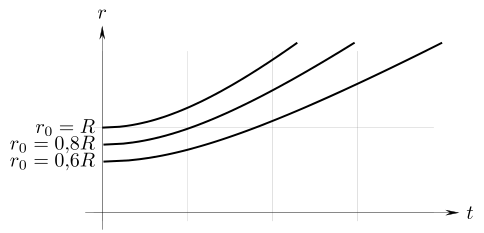
\includegraphics[width=0.5\textwidth]{images/png/sphere1.png}
\end{figure}
\\
Плотность зарядов можно найти, определяя для каждого из слоёв, между которыми находится заряд $dq$, толщина между слоями $dr_0$, в момент времени $t$ соответствующее расстояние между слоями:
$dr$:
\[
\rho = \frac{1}{4\pi r^2} \frac{dq}{dr},
\]
где $dr$ определяется $dr_0$, а $dt = 0$. В результате:
\[
	f'\left(\frac{r}{r_0}\right) \frac{dr}{r_0} = f'\left(\frac{r}{r_0}\right) \frac{r dr_0}{r_0^2} 
\]
\[
	\frac{dr}{r} = \frac{dr_0}{r_0}
\]
\[
	\rho = \frac{Q}{4\pi R^3/3} \left(\frac{r_0}{r}\right)^3 = \rho_0 \left(f^{-1}\left(\sqrt{
		\frac{2\alpha k Q}{R^{3}} } t\right)\right)^{-3}
\]
То есть $\rho$ зависит только от времени и не зависит от расстояния, что означает, что шар всегда однороден.

\textit{Второй метод}.

С точки зрения уравнений Максвелла в сферически-симметричном случае:
\[
	\begin{aligned}
		& \begin{vmatrix}
			\cfrac{1}{r^2 \sin \theta} \,\vec{e}_r & \cfrac{1}{r \sin \theta}\, \vec{e}_\theta & \cfrac{1}{r} \, \vec{e}_\alpha \\
			\df{r} & 0 & 0 \\
			E_r & r E_\theta & r \sin \theta E_\alpha
		\end{vmatrix}
		= 
		- \dff{\vec{B}}{t} \\
		& \begin{vmatrix}
		\cfrac{1}{r^2 \sin \theta} \,\vec{e}_r & \cfrac{1}{r \sin \theta}\, \vec{e}_\theta & \cfrac{1}{r} \, \vec{e}_\alpha \\
		\df{r} & 0 & 0 \\
		B_r & r B_\theta & r \sin \theta B_\alpha
		\end{vmatrix}
		= 
		\mu_0 \rho \vec{v} + \frac{1}{c^2} \dff{\vec{E}}{t} \\
		& \frac{1}{r^2} \df{r} \left( r^2 E_r\right) = \frac{\rho}{\varepsilon_0} \\ 
		& \frac{1}{r^2} \df{r} \left( r^2 B_r\right) = 0 \\
		& \left(\dff{\vec{v}}{t} + \vec{v}\cdot\nabla\vec{v}\right) = A \left(\vec{E} + 
		\begin{vmatrix}
		\vec{e}_r & \vec{e}_\theta & \vec{e}_\alpha \\
		v_r & v_\theta & v_\alpha \\
		B_r & B_\theta & B_\alpha
		\end{vmatrix} \right)
	\end{aligned}
	\Rightarrow
	\begin{aligned}
		& \dff{B_r}{t} = 0 \\
		& \dff{B_\theta}{t} = \frac{1}{r} \df{r} \left( r E_\alpha\right) \\
		& \dff{B_\alpha}{t} = - \frac{1}{r} \df{r} \left( r E_\theta\right) \\
		& \dff{E_r}{t} = - \frac{\rho v_r}{\varepsilon_0} \\
		& \dff{E_\theta}{t} = - c^2 \frac{1}{r} \df{r} \left( r B_\alpha\right) - \frac{\rho v_\theta}{\varepsilon_0} \\
		& \dff{E_\alpha}{t} = c^2\frac{1}{r} \df{r} \left( r B_\theta\right) - \frac{\rho v_\alpha}{\varepsilon_0}\\
		& \frac{1}{r^2} \df{r} \left( r^2 E_r\right) = \frac{\rho}{\varepsilon_0} \\ 
		& \frac{1}{r^2} \df{r} \left( r^2 B_r\right) = 0 \\
		& \dff{v_r}{t} = - v_r\dff{v_r}{r} + A\left(E_r + v_\theta B_\alpha - v_\alpha B_\theta\right) \\
		& \dff{v_\theta}{t} = - v_r\dff{v_\theta}{r} + A\left(E_\theta + v_\alpha B_r - v_r B_\alpha\right) \\
		& \dff{v_\alpha}{t} = - v_r\dff{v_\alpha}{r} + A\left(E_\alpha + v_r B_\theta - v_\theta B_r\right) \\
	\end{aligned}
\] 
Если в начальный момент времени:
\[
	E_\alpha, E_\theta, B_r, B_\alpha, B_\theta, v_\theta, v_\alpha, v_r = 0,
\]
то как следует из системы уравнений первого порядка по времени, во все следующие моменты времени:
\[
	E_\alpha, E_\theta, B_r, B_\alpha, B_\theta, v_\theta, v_\alpha = 0,
\]
Остаётся система из трёх уравнений:
\[
	\begin{aligned}
	& \dff{E_r}{t} = - \frac{\rho v_r}{\varepsilon_0} \\
	& \frac{1}{r^2} \df{r} \left( r^2 E_r\right) = \frac{\rho}{\varepsilon_0} \\
	& \dff{v_r}{t} = - v_r\dff{v_r}{r} + A E_r
	\end{aligned}
\]
Отсюда легко получить систему:
\[
	\begin{aligned}
	& \dff{r^2 E_r}{t} + v_r \df{r} \left( r^2 E_r\right) = 0 \\
	& \dff{v_r}{t} + v_r\dff{v_r}{r} = A E_r
	\end{aligned}
\]
Как её решать? Методом характеристик. Все уравнения имеют один и тот же вид и представляют собой уравнения переноса. Скорость переноса $v_r$. Система в методе характеристик:
\[
	\begin{aligned}
	& \Dff{r}{t} = v_r \\
	& \Dff{(r^2 E_r)}{t} = 0 \\
	& \Dff{v_r}{t} = A E_r
	\end{aligned}
\]
Из второго уравнения следует, что:
\[
	E_r = \frac{E_r(0) r_0^2}{r^2} = k\frac{r_0^3}{R^3 r^2} Q = k \frac{q}{r^2}
\]
И система сводится к системе из предыдущего метода.

\section{Влияние гравитации поля на заряженный шар}

Поле имеет энергию и следовательно массу. Резонно предположить, что эта масса должна участвовать в гравитационных взаимодействиях и гравитация поля должна влиять на движение заряженной среды. Попробуем это учесть.

В сферически симметричном случае массу поля, ограниченная сферой радиуса $r(r_0, t)$, можно найти из выражения:
\[
	m = \frac{\varepsilon_0}{2c^2} \int\limits_0^{r(r_0, t)} E_r^2 4 \pi r^2 dr = 
	\frac{4\pi k^2 \varepsilon_0 Q^2}{2c^2 R^6} \int\limits_0^{r_0} \frac{r_0^6}{r^2} \dff{r}{r_0} dr_0 =
	\frac{k Q^2}{2c^2 R^6} \int\limits_0^{r_0} \frac{r_0^6}{r^2} \dff{r}{r_0} dr_0
\]

Будем считать, что гравитация Ньютонова, случай нерелятивистский, плотность заряда и плотность массы пропорциональны:
\[
	\alpha \rho = \rho_m
\]
Тогда получим уравнения движения:
\[
	\Dff{v_r}{t} = (A + G \alpha / k) k\frac{r_0^3}{R^3 r^2} Q + \frac{k Q^2}{2c^2 R^6} \int\limits_0^{r_0} \frac{r_0^6}{r^2} \dff{r}{r_0} dr_0
\]


\section{Метод характеристик для уравнений Максвелла}

Метод характеристик удобно применять для среды, описываемой уравнениями гидродинамики. Система уравнений Максвелла и второй закон Ньютона для заряженной жидкости с отношением заряда к массе для частицы среды $A$:
\[
	\begin{aligned}
	& \div \vec{E} = \frac{\rho}{\varepsilon_0} \\
	& \rot \vec{E} = - \dff{\vec{B}}{t}\\
	& \div \vec{B} = 0 \\
	& \rot \vec{B} = \mu_0 \rho \vec{v} + \frac{1}{c^2} \dff{E}{t} \\
	& \dff{\vec{v}}{t} + (\vec{v}\cdot\nabla) \vec{v} = \vec{a}(A(\vec{E} + \vec{v}\times\vec{B}))
	\end{aligned}
	\Rightarrow
	\begin{aligned}
	& \Dff{\vec{E}}{t} = c^2 \rot \vec{B} - \vec{v} \div \vec{E} + (\vec{v} \cdot \nabla) \vec{E} \\
	& \Dff{\vec{B}}{t} = - \rot \vec{E} + (\vec{v} \cdot \nabla) \vec{B} \\
	& \Dff{\vec{v}}{t} = \vec{a}(A(\vec{E} + \vec{v}\times\vec{B})) \\
	& \Dff{\vec{r}}{t} = \vec{v}
	\end{aligned}
\] 
\[
	\begin{aligned}
	& \Dff{\vec{E}}{t} = c^2 \nabla_B \times \vec{B} - \vec{v} (\nabla_E \cdot \vec{E}) + (\vec{v} \cdot \nabla_E) \vec{E} =
		c^2 \nabla_B \times \vec{B} - \nabla_E \times (\vec{v} \times \vec{E}) =
		c^2 \nabla_{E, B} \times \left(\vec{B} - \frac{\vec{v}}{c^2} \times \vec{E}\right) \\
	& \Dff{\vec{B}}{t} = -  \nabla_E \times \vec{E} - \vec{v} (\nabla_B \cdot \vec{B}) + (\vec{v} \cdot \nabla_B) \vec{B} =
		- \nabla_E \times \vec{E} - \nabla_B \times (\vec{v} \times \vec{B}) =
		- \nabla_{E, B} \times \left(\vec{E} + \vec{v} \times \vec{B}\right) \\
	& \Dff{\vec{v}}{t} = \vec{a}(A(\vec{E} + \vec{v}\times\vec{B})) \\
	& \Dff{\vec{r}}{t} = \vec{v}
	\end{aligned}
\]
Последняя система интересна тем, что вскрывает некоторые внутренние связи, но предыдущая система лучше поддаётся анализу. Итак,
\[
	\begin{aligned}
	& \Dff{\vec{E}}{t} = c^2 \rot \vec{B} - \vec{v} \div \vec{E} + (\vec{v} \cdot \nabla) \vec{E} \\
	& \Dff{\vec{B}}{t} = - \rot \vec{E} + (\vec{v} \cdot \nabla) \vec{B} \\
	& \Dff{\vec{v}}{t} = \vec{a}(A(\vec{E} + \vec{v}\times\vec{B})) \\
	& \Dff{\vec{r}}{t} = \vec{v}
	\end{aligned}
\]
Начальные условия:
\[
	\vec{E}(\vec{r}_0, t_0), \quad \vec{B}(\vec{r}_0, t_0),  \quad\vec{v}(\vec{r}_0, t_0), \quad \vec{r}(t_0) = \vec{r}_0
\]
Решением системы будут выражения:
\[
	\vec{E}(\vec{r}_0, t), \quad \vec{B}(\vec{r}_0, t),  \quad\vec{v}(\vec{r}_0, t), \quad \vec{r}(\vec{r}_0, t)
\]
Здесь $\vec{r}_0$ аналог постоянной интегрирования. Первые три выражения показывают как меняется электромагнитные поля и поле скоростей в различные моменты времени вдоль характеристики. Выбирая в качестве $\vec{r}_0$ все точки пространства, можно получить поле во всём пространстве в различные моменты времени.
\section{Движение заряженной частицы в скрещенных полях}
Рассмотрим движение частицы массой $m$, зарядом $q$ в скрещенном поле $\vec{E} = -\vec{u}\times\vec{B}$. Уравнения движения:
\[
	\Dff{\vec{p}}{t} = q (\vec{E} + \vec{v} \times \vec{B}) =
	q (\vec{v} - \vec{u})\times\vec{B}
\]
Вводим собственное время $\tau$:
\[
	\Dff{\tau}{t} = \sqrt{1 - v^2/c^2} = \frac{mc^2}{W}
\]
Тогда:
\[
	\Dff{\vec{p}}{\tau} =
	\frac{q}{m} (\vec{p} - \vec{u}W/c^2)\times\vec{B}
\]
Вводим циклотронную частоту:
\[
	\vec{\omega}_0 = \frac{q}{m}\vec{B}
\]
\[
	\Dff{\vec{p}}{\tau} =
	- \vec{\omega}_0\times(\vec{p} - \vec{u}W/c^2)
\]
Рассмотрим также энергию:
\[
	W = \sqrt{p^2c^2 + m^2 c^4}
\]
\[
	\Dff{W}{\tau} = \frac{c^2}{W} \vec{p}\cdot\Dff{\vec{p}}{\tau} = 
	\vec{p}\cdot(\vec{\omega}_0\times\vec{u})
\]
Заметим теперь, что:
\[
	\vec{\omega}_0 \cdot \vec{p} = \vec\omega_0 \cdot \vec{p}_0
\]
\[
	\Dff{\vec{u}\cdot\vec{p}}{\tau} = - \vec{u}\cdot(\vec{\omega}_0\times\vec{p}) = \vec{p}\cdot(\vec{\omega}_0\times\vec{u}) = \Dff{W}{\tau} 
\]
В результате:
\[	
	W - \vec{u}\cdot\vec{p} = const = W_0 - \vec{u}\cdot\vec{p}_0 = W_0'
\]
\[
	\Dff{\vec{p}}{\tau} =
	- \vec{\omega}_0\times(\vec{p} - \vec{u}(\vec{u}\cdot\vec{p})/c^2 -\vec{u} W_0'/c^2)
\]
Введём правую тройку ортов:
\[
	\vec{e}_\omega = \frac{\vec\omega_0}{\omega_0} \quad
	\vec{e}_t = \frac{\vec{e}_\omega \times \vec{u}}{|\vec{e}_\omega \times \vec{u}|} = \frac{\vec{e}_\omega \times \vec{u}}{u\sin \theta} \quad
	\vec{e}_s = \vec{e}_\omega\times\vec{e}_t = \frac{\vec{e}_\omega u \cos \theta - \vec{u}}{u\sin \theta} = \frac{\vec{e}_\omega \cos \theta - \vec{u}/u}{\sin \theta}
\]
\[
	\vec{u} = u \cos \theta \vec{e}_\omega - u \sin \theta \vec{e}_s
\]
\[
	\Dff{p_s}{\tau} \vec{e}_s + \Dff{p_t}{\tau} \vec{e}_t =
	\omega_0 p_s \vec{e}_t - 
	\omega_0 p_t \vec{e}_s - 
	\omega_0 u^2 \sin^2 \theta p_s/c^2 \vec{e}_t + 
	\omega_0 u^2 \cos \theta \sin \theta p_\omega /c^2 \vec{e}_t +
	\omega_0 u \sin \theta W_0'/c^2 \vec{e}_t
\]
\[	
	\begin{aligned}
	& p_\omega = p_{0\omega} \\
	& \Dff{p_s}{\tau} = - \omega_0 p_t \\
	& \Dff{p_t}{\tau} = \omega_0 (1 - u^2 \sin^2 \theta/c^2) p_s + \omega_0 u \sin \theta W_0'/c^2 + \omega_0 u^2 \cos \theta \sin \theta p_{0\omega} /c^2 =
	\omega_0 (1 - u^2 \sin^2 \theta/c^2) p_s + \omega_0 u \sin \theta (W_0 + u \sin \theta p_{0s})/c^2
	\end{aligned}
\]
\[	
	\Dfs{p_t}{\tau} = \omega_0^2 (u^2 \sin^2 \theta/c^2 - 1) p_\tau
\]
Введём обозначения:
\[
	k = \omega_0 \sqrt{u^2 \sin^2 \theta/c^2 - 1}
\]
\[
	\begin{aligned}
	& m\Dff{x_t}{\tau} = p_t = A \sinh (k\tau) + p_{0t} \cosh(k\tau) \\
	& m\Dff{x_s}{\tau} = p_s = - \frac{\omega_0}{k} (A \cosh (k\tau) + p_{0t} \sinh (k\tau)) + \frac{\omega_0^2 u \sin \theta (W_0 + u \sin \theta p_{0s})}{k^2 c^2} \\
	& \Rightarrow A = \frac{\omega_0 u \sin \theta (W_0 + u \sin \theta p_{0s})}{k c^2} - \frac{k}{\omega_0} p_{0s}  = 
	\frac{\omega_0 (u \sin \theta W_0/c^2 + p_{0s})}{k} \\
	& \Rightarrow p_s = - \frac{\omega_0}{k} (A (\cosh (k\tau) - 1) + p_{0t} \sinh (k\tau)) + p_{0s} \\
	& m\Dff{x_\omega}{\tau} = p_\omega = p_{0\omega} \\
	& m c^2\Dff{t}{\tau} = W = W_0 - u \sin \theta (p_s - p_{0s})
	\end{aligned}
\]
\[
	\begin{aligned}
	& x_t = \frac{1}{mk} (A (\cosh (k\tau) - 1) + p_{0t} \sinh(k\tau)) + x_{0t} \\
	& x_s = - \frac{\omega_0}{k^2m} (A (\sinh (k\tau) - k\tau) + p_{0t} (\cosh (k\tau) - 1)) + \frac{p_{0s} \tau}{m} + x_{0s} \\
	& x_\omega = \frac{p_{0\omega} \tau}{m} + x_{0\omega} \\
	& t = \frac{1}{mc^2} (W_0 \tau - u \sin \theta (m (x_s - x_{0s}) - p_{0s} \tau))
	\end{aligned}
\]
Если $u \sin \theta = c$:
\[
	\begin{aligned}
	& \qquad A = A'/k = \frac{\omega_0 (W_0/c + p_{0s})}{k}\\
	& x_t = \frac{1}{m} (A'\frac{\tau^2}{2} + p_{0t} \tau) + x_{0t} \\
	& x_s = - \frac{\omega_0}{m} \left(A' \frac{\tau^3}{6} + p_{0t} \frac{\tau^2}{2}\right) + \frac{p_{0s} \tau}{m} + x_{0s} \\
	& x_\omega = \frac{p_{0\omega} \tau}{m} + x_{0\omega} \\
	& t = \frac{1}{mc^2} (W_0 \tau - u \sin \theta (m (x_s - x_{0s}) - p_{0s} \tau))
	\end{aligned}
\]
Если $u \sin \theta < c$:
\[
	\begin{aligned}
	& \qquad k = i \omega \qquad A = - i A'\\
	& x_t = \frac{1}{m\omega} (- A' (\cos (\omega\tau) - 1) + p_{0t} \sin(\omega\tau)) + x_{0t} \\
	& x_s = \frac{\omega_0}{\omega^2m} (A' (\sin (\omega \tau) - \omega \tau) + p_{0t} (\cos (\omega \tau) - 1)) + \frac{p_{0s} \tau}{m} + x_{0s} \\
	& x_\omega = \frac{p_{0\omega} \tau}{m} + x_{0\omega} \\
	& t = \frac{1}{mc^2} (W_0 \tau - u \sin \theta (m (x_s - x_{0s}) - p_{0s} \tau))
	\end{aligned}
\]

\section{Движение частицы в материальной среде в нерелятивистском случае}

Рассмотрим материальную среду, частицы которой не взаимодействуют между собой. Уравнения движения для такой среды будут иметь вид уравнений Эйлера с нулевой правой частью:
\[
	\rho \Dff{\vec{v}}{t} = \rho \left(\dff{\vec{v}}{t} + (\vec{v}\cdot\nabla) \vec{v}\right) = 0
\]
\[
	\dff{\rho}{t} + \div (\rho \vec{v}) = 0
\]
То, что в среде находится частица учтём с помощью выражения:
\[
	\rho = \rho_f + m \delta(\vec{r} - \vec{\xi}(t))
\]
Из уравнения непрерывности следует:
\[
	\dff{\rho_f}{t} + \div (\rho_f \vec{v}) 
	- m \Dff{\vec{\xi}}{t} \cdot \nabla\delta(\vec{r} - \vec{\xi}(t)) 
	+ m \vec{v} \cdot \nabla\delta(\vec{r} - \vec{\xi}(t)) 
	+ m \delta(\vec{r} - \vec{\xi}(t)) \div{\vec{v}} = 0
\]
Можно предположить (к сожалению мне это казалось абсолютно точным, но вдруг я где-то ошибся), что отсюда следует:
\[
	\dff{\rho_f}{t} + \div (\rho_f \vec{v}) = 0
\]
\[
	\div \vec{v} = 0 \text{ но только в точке с частицей}
\]
\[
	\vec{v} = \Dff{\vec{\xi}}{t} \text{ но только в точке с частицей}
\]
Разделяем выражения и интегрируем по $\vec{r}$, учитывая, что на $\vec{r} = \vec{\xi}(t)$ $\vec{v} = d\vec{\xi}/dt$:
\[
	m\Dfs{\vec{\xi}}{t} = - \int \rho_f \left(\dff{\vec{v}}{t} + (\vec{v}\cdot\nabla) \vec{v}\right) dV
\]
На деле как легко видеть скорости частиц не меняются при движении, если поле скоростей непрерывно. Интерес представляет один единственный случай, когда поле скоростей терпит разрыв. В этом случае частица догоняет и сталкивается с частицами среды и, как следствие, движется уже ускоренно. Здесь есть несколько важных и нетривиальных моментов. Очень хочется, чтобы разрыв был в одной единственной точке -- в точке с частицей. Но если разрыв конечен, то для частицы как материальной точки производные от скорости обратятся в нуль и ничего не будет наблюдаться. Если предположить, что в среде существует фронт или линия на которой поле скоростей терпит разрыв, то расположение этой линии или фронта может быть вообще говоря произвольным. Это путает все карты.
Как облечь всё изложенное выше в математическую форму я пока не знаю. По этой причине на задачу пришлось забить.
\section{Волновые уравнения}
\subsection{Однородное одномерное волновое уравнение в неограниченной среде с заданными начальными условиями}

Как оно выглядит? Да, вот так:
\[
	\dfs{u}{x} - \frac{1}{v^2} \dfs{u}{t} = 0
\]
В обычном случае $v = const$. Начальные условия:
\[
	\begin{aligned}
		& u(0, x) = f(x) \\
		& \dff{u}{t} \Big|_{(0, x)} = g(x)
	\end{aligned}
\]
Его очень легко решить, если воспользоваться заменой координат:
\[
	\begin{aligned}
	& \eta = x + v t \\
	& \xi = x - v t
	\end{aligned}	
\]
\[
	\begin{aligned}
		& \dff{u}{x} = \dff{u}{\eta} \dff{\eta}{x} + \dff{u}{\xi} \dff{\xi}{x} =
			\dff{u}{\eta} + \dff{u}{\xi} \\
		& \dfs{u}{x} = \dfs{u}{\eta} \dff{\eta}{x} + \dfss{u}{\xi}{\eta} \dff{\xi}{x} + \dfss{u}{\eta}{\xi} \dff{\eta}{x} +  \dfs{u}{\xi} \dff{\xi}{x} =
			\dfs{u}{\eta} +  \dfs{u}{\xi} + 2 \dfss{u}{\xi}{\eta} \\
		& \dff{u}{t} = \dff{u}{\eta} \dff{\eta}{t} + \dff{u}{\xi} \dff{\xi}{t} =
			v \left(\dff{u}{\eta} - \dff{u}{\xi}\right) \\
		& \dfs{u}{t} = v\dfs{u}{\eta} \dff{\eta}{t} + v\dfss{u}{\xi}{\eta} \dff{\xi}{t} - v\dfss{u}{\eta}{\xi} \dff{\eta}{t} -  v\dfs{u}{\xi} \dff{\xi}{t} =
		v^2\left(\dfs{u}{\eta} +  \dfs{u}{\xi} - 2 \dfss{u}{\xi}{\eta} \right)\\ 
	\end{aligned}
\]
\[
	\dfs{u}{x} - \frac{1}{v^2} \dfs{u}{t} = 4 \dfss{u}{\xi}{\eta} = 0
\]
\[
	\dff{u}{\eta} = U_1(\eta)
\]
\[
	u = U(\eta) + V(\xi)
\]
\[
	\begin{aligned}
	& u(0, x) = U(x) + V(x) = f(x) \\
	& \dff{u}{t} \Big|_{(0, x)} = v \left(U'(x) - V'(x)\right) = g(x)
	\end{aligned}
	\Rightarrow
	\begin{aligned}
	& U(x) + V(x) = f(x) \\
	& U(x) - V(x) = \frac{1}{v} \int g(x) dx = \frac{G(x)}{v}
	\end{aligned}
\]
\[
	u = \frac{f(x + v t) + f(x - v t)}{2} + \frac{G(x + v t) - G(x - v t)}{2 v} = \frac{f(x + v t) + f(x - v t)}{2} + \frac{1}{2 v} \int\limits_{x - v t}^{x + v t} g(x) dx
\]

\subsection{Метод преобразования Фурье для неоднородного одномерного волнового уравнения в бесконечной среде с нулевыми начальными условиями}

\[
\dfs{u}{x} - \frac{1}{v^2} \dfs{u}{t} = s(x, t)
\]
$v = const$. Начальные условия:
\[
	\begin{aligned}
	& u(0, x) = 0 \\
	& \dff{u}{t} \Big|_{(0, x)} = 0
	\end{aligned}
\]
Только координата $x$ меняется от $-\infty$ до $\infty$, поэтому преобразование Фурье будет иметь вид:
\[
	\begin{aligned}
	& u(x, t) = \int\limits_{-\infty}^{\infty} U(k, t) e^{-ikx} dk \qquad\Leftrightarrow \qquad  U(k, t) = \frac{1}{2\pi}\int\limits_{-\infty}^{\infty} u(x, t) e^{ikx} dx\\
	& s(x, t) = \int\limits_{-\infty}^{\infty} S(k, t) e^{-ikx} dk
	\qquad\Leftrightarrow \qquad
	S(k, t) = \frac{1}{2\pi}\int\limits_{-\infty}^{\infty} s(x, t) e^{ikx} dx
	\end{aligned}
\]
Выполняем преобразование Фурье исходного уравнения:
\[
	\frac{1}{2\pi} \int\limits_{-\infty}^{\infty}\dfs{u}{x} e^{ikx} dx = 
	\frac{1}{2\pi} \dff{u}{x} e^{ikx} \Big|_{-\infty}^{\infty} - 
	\frac{ik}{2\pi} \int\limits_{-\infty}^{\infty}\dff{u}{x} e^{ikx} dx =
	\frac{1}{2\pi} \left(\dff{u}{x} - ik u \right) e^{ikx} \Big|_{-\infty}^{\infty}
	- k^2 U
\]
При условии, что:
\[
	 \lim\limits_{x \to \pm \infty }\left(\dff{u}{x} - ik u \right) = 0
\]
получаем преобразованное уравнение:
\[
	- k^2 U - \frac{1}{v^2} \Dfs{U}{t} = S(k, t)
\]
И начальные условия:
\[
	\begin{aligned}
	& U(k, 0) = 0 \\
	& \Dff{U}{t} \Big|_{(k, 0)} = 0
	\end{aligned}
\]
Решение этого уравнения:
\[
	U(k, t) = - \frac{v}{k} \int\limits_{0}^{t} \sin(vk (t - t')) S(k, t') dt'
\]
\[
	\begin{gathered}
	u(x, t) = -\int\limits_{0}^{t} \! \int\limits_{-\infty}^{\infty} \frac{v}{k} \sin(vk (t - t')) S(k, t') e^{-ikx}  dk\, dt' =
	-\int\limits_{0}^{t} \! \int\limits_{-\infty}^{\infty} \! \int\limits_{-\infty}^{\infty} \frac{v}{2k\pi} \sin(vk (t - t')) s(x', t') e^{-ik(x - x')}  dk\, dt'\, dx' = \\ =
	-\frac{v}{4} \int\limits_{0}^{t}  \! \int\limits_{-\infty}^{\infty} [ \sign (x - x' + v(t - t')) - \sign (x - x' - v (t - t')) ] s(x', t') dt' dx' = \\ =
	-\frac{v}{4} \int\limits_{0}^{t} \! \int\limits_{-\infty}^{\infty} [ \sign (\xi + v \tau) - \sign (\xi - v\tau) ] s(x - \xi, t - \tau) d\tau d\xi 
	\end{gathered}
\]
\[
	\begin{aligned}
	\sign (x + a) - \sign (x - a) = 
	\begin{cases}
	\left\{
	\begin{aligned}
	& 0, & x > a, \\
	& 1, & x = a, \\
	& 2, & -a < x < a, \\
	& 1, & x = - a, \\
	& 0, & x < - a.
	\end{aligned}
	\right\},
	& a > 0, \\
	0,
	& a = 0, \\
	\left\{
	\begin{aligned}
	& 0, & x > - a, \\
	& -1, & x = - a, \\
	& -2, & a < x < -a, \\
	& -1, & x = a, \\
	& 0, & x < a.
	\end{aligned}
	\right\},
	& a < 0. \\
	\end{cases}
	=
	\begin{cases}
	0, & |x|>|a|, \\ 
	\sign(a), & |x|=|a|, \\ 
	2 \sign(a), & |x| < |a|.
	\end{cases}
	=
	2 \eta(|a| - |x|) \sign(a)
	\end{aligned}
\]
\[
	 \sign (\xi + v \tau) - \sign (\xi - v\tau) = 2 \eta(v|\tau| - |\xi|) \sign(v\tau)
\]
\[
	\begin{aligned}
	u(x, t) =
	-\frac{v}{2} \int\limits_{0}^{t} \! \int\limits_{-\infty}^{\infty} \eta(v|\tau| - |\xi|) \sign(v\tau) s(x - \xi, t - \tau) d\tau\, d\xi = \\ =
	[\text{если, $s(x - \xi, t - \tau)$ не имеет $\delta$-образных разывов}] = \\ =
	-\frac{v}{2} \int\limits_{0}^{t} \! \int\limits_{-v\tau}^{v\tau} s(x - \xi, t - \tau) d\tau\, d\xi
	\end{aligned}
\]
%Проверим, что найденное решение удовлетворяет уравнению:
%\[
%	\begin{gathered}
%	\dfs{u}{x} - \frac{1}{v^2} \dfs{u}{t} =
%	-\frac{v}{2} \int\limits_{0}^{t} \! \int\limits_{-\infty}^{\infty} \eta(\tau - |\xi|/v)
%	\left(\dfs{}{x} - \frac{1}{v^2} \dfs{}{t}\right) s(x - \xi, t - \tau) d\tau\, d\xi = \\ =
%	-\frac{v}{2} \int\limits_{0}^{t} \! \int\limits_{-\infty}^{\infty} \eta(\tau - |\xi|/v)
%	\left(\dfs{}{\xi} - \frac{1}{v^2} \dfs{}{\tau}\right) s(x - \xi, t - \tau) d\tau\, d\xi
%	\end{gathered}
%\]

\subsection{Примеры}

\textbf{1. Пусть:}
\[
s(x, t) = \delta(x - x_0) \delta (t - t_0) 
\]
что соответствует импульсу, мгновенно переданному отдельной точке струны.
\[
\begin{gathered}
u(x, t) =
-\frac{v}{4} \int\limits_{0}^{t} \! \int\limits_{-\infty}^{\infty} [ \sign (\xi + v \tau) - \sign (\xi - v\tau) ] s(x - \xi, t - \tau) d\tau d\xi =
\\ =
-\frac{v}{4} \int\limits_{0}^{t} \! \int\limits_{-\infty}^{\infty} [ \sign (\xi + v \tau) - \sign (\xi - v\tau) ] \delta(x - x_0 - \xi) \delta (t - t_0 - \tau)  d\tau d\xi =
\\ =
-\frac{v}{4} \int\limits_{0}^{t}  [ \sign (x - x_0 + v \tau) - \sign (x - x_0 - v\tau) ] \delta (t - t_0 - \tau)  d\tau = 
\\ =
-\frac{v}{4} [ \sign (x - x_0 + v (t - t_0)) - \sign (x - x_0 - v(t - t_0)) ] \eta(t - t_0)
\end{gathered}
\]
Проверяем:
\[
\dfs{u}{x} = - \frac{v}{2} [\delta' (x - x_0 + v (t - t_0)) - \delta' (x - x_0 - v(t - t_0))]\eta(t - t_0)
\]
\[
\begin{gathered}
\dfs{u}{t} = -\frac{v}{4} \left\{
2 v^2 [\delta' (x - x_0 + v (t - t_0)) - \delta' (x - x_0 - v(t - t_0)) ] \eta(t - t_0) +
\right.\\ + \left.
4 v [\delta (x - x_0 + v (t - t_0)) + \delta (x - x_0 - v(t - t_0))]\delta(t - t_0) +
\right.\\ + \left.
[ \sign (x - x_0 + v (t - t_0)) - \sign (x - x_0 - v(t - t_0)) ] \delta'(t - t_0)
\right\}
\end{gathered}
\]
Воспользуемся тождествами:
\[
f(x)\delta(x - x_0) + [F(x) - F(x_0)] \delta'(x - x_0) = 0, \qquad F(x) = \int f(x) dx
\]
\[
f(x) \delta(x -x_0) = f(x_0) \delta(x - x_0)
\]
Кое-что подсократилось:
\[
\begin{gathered}
\dfs{u}{t} = -\frac{v}{4} \left\{
2 v^2 [\delta' (x - x_0 + v (t - t_0)) - \delta' (x - x_0 - v(t - t_0)) ] \eta(t - t_0) +
\right.\\ + \left.
4 v \delta (x - x_0) \delta(t - t_0)
\right\}
\end{gathered}
\]
\[
\Rightarrow
\dfs{u}{x} - \frac{1}{v^2} \dfs{u}{t} = \delta (x - x_0) \delta(t - t_0)
\]
На рисунке показан профиль струны в различные моменты времени:
\begin{center}
	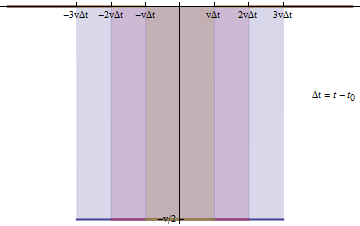
\includegraphics[width=0.5\textwidth]{images/png/for_delta_force.png}
\end{center}

\textbf{Одно тождество}

Рассмотрим функцию вида:
\[
	u(x, t) = \eta(t - t_0) \eta(\xi) f(\xi) = g(\xi, t) f(\xi), \text{ если } \xi = |t - t_0| - |x - x_0|/v 
\]
\[
	\begin{gathered}
	u''_{tt} = 
	\dfs{g}{t} f + 2 \dff{g}{t} \dff{f}{\xi} \dff{\xi}{t} + g \dfs{f}{t} 
	\end{gathered}
\]
\[
	\begin{gathered}
	u''_{xx} = 
	\dfs{g}{x} f + 2 \dff{g}{x} \dff{f}{\xi} \dff{\xi}{x} + g \dfs{f}{x} 
	\end{gathered}
\]
\[
	\begin{gathered}
	u''_{xx} - \frac{1}{v^2} u''_{tt} = 
	f\left(\dfs{g}{x} - \frac{1}{v^2} \dfs{g}{t} \right) + 
	2 \dff{f}{\xi} \dff{g}{\xi} \left[\left(\dff{\xi}{x}\right)^2 - \frac{1}{v^2} \left(\dff{\xi}{t}\right)^2 \right] -
	\frac{2}{v^2} \delta(t - t_0) \eta (\xi) \dff{f}{\xi} \dff{\xi}{t} + 
	\\ +
	g\left[\df{x} \left(\dff{f}{\xi} \dff{\xi}{x} \right) - \frac{1}{v^2} \df{t} \left(\dff{f}{\xi} \dff{\xi}{t} \right)  \right]
	= 
	\\ =
	f\left(\dfs{g}{x} - \frac{1}{v^2} \dfs{g}{t} \right) + 
	2 \dff{f}{\xi} \dff{g}{\xi} \left[\left(\dff{\xi}{x}\right)^2 - \frac{1}{v^2} \left(\dff{\xi}{t}\right)^2 \right] -
	\frac{2}{v^2} \delta(t - t_0) \eta (\xi) \dff{f}{\xi} \dff{\xi}{t} + 
	\\ +
	g\dfs{f}{\xi} \left[\left(\dff{\xi}{x}\right)^2 - \frac{1}{v^2} \left(\dff{\xi}{t}\right)^2 \right] +
	g \dff{f}{\xi} \left(\dfs{\xi}{x} - \frac{1}{v^2} \dfs{\xi}{t} \right)
	\end{gathered}
\]
\[
	\dfs{g}{x} - \frac{1}{v^2} \dfs{g}{t} = - \frac{2}{v} \delta(t - t_0) \delta(x - x_0) \quad \text{(см. пред. пример)}
\]
\[
	\begin{aligned}
	& \dff{\xi}{t} = \sign(t - t_0) & \dff{\xi}{x} = - \sign(x - x_0) \frac{1}{v} \\
	& \dfs{\xi}{t} = 2\delta(t - t_0) & \dfs{\xi}{x} = - 2\delta(x - x_0) \frac{1}{v} \\
	\end{aligned}
\]
\[
	 \begin{gathered}
	 \dff{g}{\xi} \left[\left(\dff{\xi}{x}\right)^2 - \frac{1}{v^2} \left(\dff{\xi}{t}\right)^2 \right] =
	 \eta(t - t_0) \delta(\xi) \frac{1 - 2 \eta(-|x - x_0|) - 1 + 2 \eta(-|t - t_0|)}{v^2} =
	 \\ =
	 \frac{2\eta(t - t_0)}{v^2} (\delta(-|x - x_0|/v) \eta(-|t - t_0|) - \delta(\xi) \eta(-v|t - t_0|) ) = 0
	 \end{gathered}
\]
\[
	\delta(t - t_0) \dff{\xi}{t} = \delta(t - t_0) \sign(t - t_0)  = 0
\]
\[
	\begin{gathered}
	g\left[\left(\dff{\xi}{x}\right)^2 - \frac{1}{v^2} \left(\dff{\xi}{t}\right)^2 \right] =
	\frac{2\eta(t - t_0)}{v^2} (\eta(-|x - x_0|/v) \eta(-|t - t_0|) - \eta(|t - t_0|) \eta(-|x - x_0|) ) =
	\\ =
	- \frac{2\eta(t - t_0)}{v^2} \eta(-|x - x_0|/v) \sign^2(t - t_0)
	\end{gathered}
\]
\[
	\begin{gathered}
	g \left(\dfs{\xi}{x} - \frac{1}{v^2} \dfs{\xi}{t} \right) = 
	- \eta(t - t_0) \eta(\xi) \frac{2}{v^2} \left(\delta((x - x_0)/v) + \delta(t - t_0) \right) =
	\\ =
	- \frac{2}{v^2} \left(\eta^2(t - t_0) \delta((x - x_0)/v) + \frac{1}{2} \eta(-|x - x_0|/v)\delta(t - t_0) \right) =
	\\ =
	- \frac{2}{v^2} \left(\eta(t - t_0) \delta((x - x_0)/v) - \frac{1}{2} \eta(-|t - t_0|) \delta((x - x_0)/v)  + \frac{1}{2} \eta(-|x - x_0|/v)\delta(t - t_0) \right) =
	\\ =
	[\text{чуть выше такое уже встречалось}] =
	- \frac{2}{v} \eta(t - t_0) \delta(x - x_0)
	\end{gathered}
\]
В результате:
\[
	u''_{xx} - \frac{1}{v^2} u''_{tt}  = - \frac{2}{v} f(0) \delta(t - t_0) \delta(x - x_0) -
	f''(|t - t_0|) \frac{\eta(t - t_0)}{v^2} \sign^2(t - t_0) \eta(-|x - x_0|) -
	\frac{2}{v} f'(|t - t_0|) \eta(t - t_0) \delta(x - x_0)
\]

Здесь следует отметить одну деталь: результат имеет вид:
\[
	A\delta(x) + B\eta(-|x|)
\]
Из интегрального определения $\delta-$функции:
\[
	A\delta(x) + B\eta(-|x|) = A\delta(x)
\]
И
\[
	u''_{xx} - \frac{1}{v^2} u''_{tt}  = - \frac{2}{v} f(0) \delta(t - t_0) \delta(x - x_0) -
	\frac{2}{v} f'(|t - t_0|) \eta(t - t_0) \delta(x - x_0)
\]

\textbf{2. Пусть:}
\[
s(x, t) = \delta(x - x_0) \eta(t - t_0)
\]
что соответствует постоянной во времени силе, действующей в фиксированной точке струны, начиная с некоторого момента.
\[
\begin{gathered}
u(x, t) =
-\frac{v}{4} \int\limits_{0}^{t} \! \int\limits_{-\infty}^{\infty} [ \sign (\xi + v \tau) - \sign (\xi - v\tau) ]  \delta(x - x_0 - \xi) \eta(t - t_0 - \tau) d\tau d\xi =
\\ =
-\frac{v}{4} \int\limits_{0}^{t} [ \sign (x - x_0 + v \tau) - \sign (x - x_0 - v\tau) ] \eta (t - t_0 - \tau)  d\tau =
\\ =
-\frac{v}{4} \eta(t - t_0) \int\limits_{0}^{t - t_0} [ \sign (x - x_0 + v \tau) - \sign (x - x_0 - v\tau) ] d\tau = 
-\frac{v}{4} \eta(t - t_0) \int\limits_{0}^{t - t_0} 2 \eta(v|\tau| - |x - x_0|) d\tau =
\\ =
-\frac{v}{4} \eta(t - t_0) \eta(t - t_0 - |x - x_0|/v) \int\limits_{|x - x_0|/v}^{t - t_0} 2 \eta(v\tau - |x - x_0|) d\tau = 
-\frac{v}{2} \eta(t - t_0) \eta(t - t_0 - |x - x_0|/v) \int\limits_{|x - x_0|/v}^{t - t_0} d\tau =
\\ =
-\frac{v}{2} \eta(t - t_0) \eta(t - t_0 - |x - x_0|/v) (t - t_0 - |x - x_0|/v) 
\end{gathered}
\]
Проверка по формуле выше показывает, что это правильный ответ. Форма струны в различные моменты времени показана на рисунке:
\begin{center}
	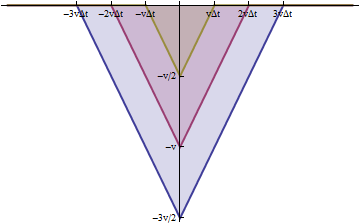
\includegraphics[width=0.5\textwidth]{images/png/for_deltac_force.png}
\end{center}

\textbf{3. Пусть:}
\[
	s(x, t) = \begin{cases}
	0, & x \notin [-l/2, l/2] \\
	S_0\eta(t - t_0)/l, & x \in [-l/2, l/2]
	\end{cases} =
	\frac{S_0}{l} [ \eta(x + l/2) - \eta(x - l/2)] \eta(t - t_0)
\]
что соответствует постоянной силе, действующей на участок струны.
\[
\begin{gathered}
	u(x, t) =
	-\frac{v}{2} \int\limits_{0}^{t} \! \int\limits_{-v\tau}^{v\tau} s(x - \xi, t - \tau) d\tau\, d\xi = 
	\\ =
	-\frac{v}{2} \int\limits_{0}^{t} \! \int\limits_{-v\tau}^{v\tau} \frac{S_0}{l} [ \eta(x + l/2 - \xi) - \eta(x - l/2 - \xi)]\eta(t - t_0 - \tau) d\tau\, d\xi = 
	\\ =
	-\frac{v}{2} \int\limits_{0}^{t - t_0} \! \int\limits_{-v\tau}^{v\tau} \frac{S_0}{l} [ \eta(x + l/2 - \xi) - \eta(x - l/2 - \xi)] d\tau\, d\xi = 
	-\frac{v}{2}\frac{S_0}{l} \int\limits_{S} d\tau\, d\xi
\end{gathered}
\]
Область интегрирования $S$ приведена на рисунке, и представляет собой пересечение полосы шириной $l$ и треугольника, ограниченного кривыми $y = v(t - t_0)$, $y = x$, $y = -x$.
\begin{center}
	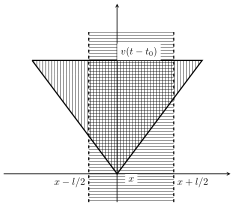
\includegraphics{images/png/for_example3.png}
	%\usetikzlibrary{patterns}
\begin{tikzpicture}

\draw[thick,-stealth]  (0,-1) -- (0,6);
\draw[thick,-stealth] (-4,0) -- (4,0);
\draw[very thick, pattern=vertical lines] (-3,4) -- (3, 4) -- (0,0) -- (-3, 4);
\draw[very thick, dashed] (2, -1) -- (2, 5);
\draw[very thick, dashed] (-1, -1) -- (-1, 5);
\path[pattern=horizontal lines] (2, -1) rectangle (-1, 5);

\node[below, fill = white] at (0.5,0) {$x$};
\node[above right, fill = white] at (0,4) {$v(t - t_0)$};
\node[below left] at (-1,0) {$x - l/2$};
\node[below right] at (2,0) {$x + l/2$};

\end{tikzpicture}
\end{center}
Решение можно представить с помощью функций, определяющих площадь пересечения треугольника с левой полуплоскостью, заданной прямой параллельной оси ординат:
\[
\begin{aligned}
& S_+(x, x_A, x_B, x_C, y_B) =  
\frac{1}{2} y_B \frac{(x - x_A)^2}{x_B - x_A} \eta(x - x_A) \eta(x_B - x)  + \\ & +
\frac{1}{2} y_B \left[(x_B - x_A) + \frac{2 x_C - x - x_B}{x_C - x_B} (x - x_B)\right] \eta(x - x_B) \eta(x_C - x) +
\frac{1}{2} y_B (x_C - x_A) \eta(x - x_C)
\end{aligned}
\]
\[
	\begin{aligned}
	u(x, t) & = -\frac{v}{2}\frac{S_0}{l} [S_+(x + l/2, -v(t - t_0), 0, v(t-t_0), v(t - t_0)) - S_+(x - l/2, -v(t - t_0), 0, v(t-t_0), v(t - t_0))]
	\end{aligned}
\]
К сожалению, выражение слишком громоздко, и его трудно проверить. На рисунке приведена форма струны в различные моменты времени:
\begin{center}
	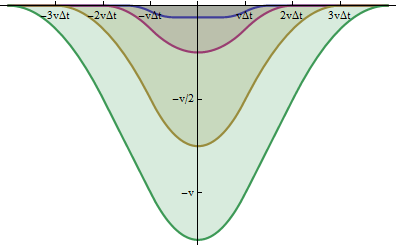
\includegraphics[width=0.5\textwidth]{images/png/for_const_force.png}
\end{center}
Примечательно, что сначала график пологий, но со временем приобретает более параболическую форму.

\textbf{4. Пусть:}

\[
s(x, t) = \delta(x - x_0) e^{i\omega t} \eta(t - t_0)
\]
что соответствует силе действующей в точке по синусоидальному закону.
\[
\begin{gathered}
u(x, t) =
-\frac{v}{4} \int\limits_{0}^{t} \! \int\limits_{-\infty}^{\infty} [ \sign (\xi + v \tau) - \sign (\xi - v\tau) ] s(x - \xi, t - \tau) d\tau d\xi =
\\ =
-\frac{v}{4} \int\limits_{0}^{t} \! \int\limits_{-\infty}^{\infty} [ \sign (\xi + v \tau) - \sign (\xi - v\tau) ] \delta(x - x_0 - \xi) e^{i\omega(t - \tau)} \eta(t - t_0 - \tau) d\tau d\xi =
\\ =
-\frac{v}{2} \eta(t - t_0) \int\limits_{0}^{t - t_0} \eta(v\tau - |x - x_0|) e^{i\omega(t - \tau)} d\tau =
-\frac{v}{2} \eta(t - t_0) \eta(t - t_0 - |x -x_0|/v) e^{i\omega t} \int\limits_{|x - x_0|/v}^{t - t_0} e^{-i\omega\tau} d\tau =
\\ =
\frac{v}{2i\omega} \eta(t - t_0) \eta(t - t_0 - |x -x_0|/v) e^{i\omega t} e^{-i\omega(t - t_0 - |x - x_0|/v)} =
\frac{v}{2i\omega} \eta(t - t_0) \eta(t - t_0 - |x -x_0|/v) \left(e^{i\omega t_0} - e^{i\omega(t - |x - x_0|/v)} \right)
\end{gathered}
\]
Как легко видеть, ответ правильный. Действительная часть:
\[
	u(x, t) = \frac{v}{2\omega} \eta(t - t_0) \eta(t - t_0 - |x -x_0|/v) \left(\sin (\omega t_0) - \sin(\omega(t - |x - x_0|/v)) \right)
\]
Форма в различные моменты времени представлена на рисунке:
\begin{center}
	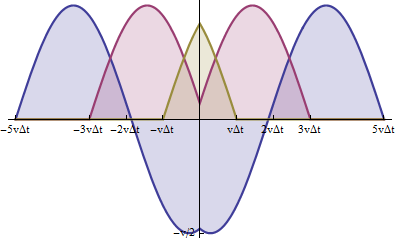
\includegraphics[width=0.5\textwidth]{images/png/for_sin_force.png}
\end{center}

\subsection{Вариационный принцип}

Рассмотрим функционал:
\[
	J(u) = \int\limits_{R^2} \left[\frac{1}{v^2} \left(\dff{u}{t}\right)^2 - \left(\dff{u}{x}\right)^2 \right] dx\, dt  
\]
\[
	\begin{gathered}
	\delta \left[\frac{1}{v^2} \left(\dff{u}{t}\right)^2 - \left(\dff{u}{x}\right)^2 \right] = 
	2 \left[\frac{1}{v^2} \dff{u}{t} \dff{\delta u}{t}  - \dff{u}{x} \dff{\delta u}{x} \right] =
	2 \left[\frac{1}{v^2} \df{t} \left(\dff{u}{t} \delta u \right)  - \df{x} \left(\dff{u}{x} \delta u \right) \right] -
	2 \left[\frac{1}{v^2} \dfs{u}{t} - \dfs{u}{x}\right] \delta u
	\end{gathered}
\]
\[
	\Rightarrow \quad \frac{1}{v^2} \dfs{u}{t} - \dfs{u}{x} = 0
\]
Для функционала:
\[
	J(u) = \int\limits_{R^2} \left[\frac{1}{v^2} \left(\dff{u}{t}\right)^2 - \left(\dff{u}{x}\right)^2 - 2 s(x, t) u \right] dx\, dt
\]
\[
	\frac{1}{v^2} \dfs{u}{t} - \dfs{u}{x} = s(x, t)
\]
Выполним преобразование Фурье:
\[
	u = u^* = \int\limits_{R^2} U(k, \omega) e^{i(\omega t - k x)} dk\, d\omega
	\qquad
	s = s^* = \int\limits_{R^2} S(k, \omega) e^{i(\omega t - k x)} dk\, d\omega
\]
\[
	\begin{gathered}
	J(U) = 
	\\ =
	\int\limits_{R^2} 
	\int\limits_{R^2}
	\int\limits_{R^2}
	\left[\frac{1}{v^2} \omega \omega' U^*(k, \omega) U(k', \omega') - k k' U^*(k, \omega) U(k', \omega') - 2 S^*(k, \omega) U(k', \omega') \right]
	e^{i((\omega' - \omega) t - (k' - k) x)}  dk\, d\omega\, dk'\, d\omega'\, dx\, dt
	=
	\\ =
	2\pi 
	\int\limits_{R^2} 
	\int\limits_{R^2}
	\left[\frac{1}{v^2} \omega \omega' U^*(k, \omega) U(k', \omega') - k k' U^*(k, \omega) U(k', \omega') - 2 S^*(k, \omega) U(k', \omega') \right]
	\delta(\omega' - \omega) \delta(k' - k) dk\, d\omega\, dk'\, d\omega'
	=
	\\ =
	2\pi 
	\int\limits_{R^2} 
	\left[\frac{1}{v^2} \omega^2 U^*(k, \omega) U(k, \omega) - k^2 U^*(k, \omega) U(k, \omega) - 2 S^*(k, \omega) U(k, \omega) \right]
	dk\, d\omega
	\end{gathered}
\]

\subsection{Решение n-мерного волнового уравнения с дельтообразной правой частью}

Волновое уравнение с дельтообразной правой частью в бесконечном пространстве-времени чудесная вещь:
\[
	\Delta u - \frac{\partial^2 u}{\partial t^2} = \delta(t - t')\delta(\vec{r} - \vec{r}') 
\]
Выполняем преобразование Фурье:
\[
	u = \int U(\vec{k}, \omega) e^{i(\vec{k}\cdot\vec{r} - \omega t)} dV_k dt
\]
Введём обозначения:
\[
	\vec{R} = \vec{r} - \vec{r}' \quad T = t - t'
\]
\[
	\delta(\vec{R}) \delta(T) = \frac{1}{(2\pi)^{n + 1}} \int e^{i(\vec{k}\cdot\vec{R} - \omega T)} dV_k d\omega
\]
Решение уравнения:
\[
	u = \frac{1}{(2\pi)^{n + 1}} \int \frac{e^{i(\vec{k}\cdot\vec{R} - \omega T)}}{\omega^2 - k^2} dV_k d\omega =  
	\frac{\pi^{(- n - 3)/2}}{2^n\Gamma\left(\frac{n - 1}{2}\right)} 
	\int\limits_{-\infty}^{\infty}\!
	\int\limits_{0}^{\infty}\!
	\int\limits_{0}^{\pi}
	 \frac{e^{i(k R \cos \theta - \omega T)}}{\omega^2 - k^2} k^{n - 1} \sin^{n - 2} \theta\, d\theta\, dk\, d\omega = (*)
\]
\[
	\frac{1}{\omega^2 - k^2} = \frac{1}{2k} \left(\frac{1}{\omega - k} - \frac{1}{\omega + k} \right)
\]
\[
	\begin{gathered}
	(*) =
	\frac{i \pi^{(- n - 1)/2}}{2^{n + 1}\Gamma\left(\frac{n - 1}{2}\right)} 
	\int\limits_{0}^{\infty}\!
	\int\limits_{0}^{\pi}
	\left(e^{ - i k T}  - e^{i k T} \right) \sign(-T)
	e^{i(k R \cos \theta)} 
	k^{n - 2} \sin^{n - 2} \theta\, d\theta\, dk
	= \\ =
	\frac{\pi^{(- n - 1)/2}}{2^{n}\Gamma\left(\frac{n - 1}{2}\right)} 
	\int\limits_{0}^{\infty}\!
	\int\limits_{0}^{\pi}
	\sin (kT) \sign(-T)
	e^{i(k R \cos \theta)} 
	k^{n - 2} \sin^{n - 2} \theta\, d\theta\, dk
	\end{gathered} 
\]
\section{Колебания с произвольной возбуждающей силой}

Уравнение колебаний:
\[
	\ddot{x} + \omega_0^2 x = f(t)
\]
\[
	x(0) = x_0, \quad \dot{x}(0) = \dot{x}_0
\]
Решение будем искать в классе непрерывных функций. Рассмотрим вспомогательную задачу:
\[
	\ddot{y} + \omega_0^2 y = \eta(t - t')
\]
\[
	y(0) = 0, \quad \dot{y}(0) = 0 \quad t' > 0
\]
Её решение с непрерывной первой производной, как легко убедиться простой подстановкой:
\[
	y = 
	\begin{cases}
	0 & t<t' \\
	\frac{1 - \cos(\omega_0 (t - t'))}{\omega_0^2} & t \geqslant t'
	\end{cases}
\]
Тогда решением задачи:
\[
	\ddot{z} + \omega_0^2 z = \delta(t - t')
\]
\[
	z(0) = 0, \quad \dot{z}(0) = 0 \quad t' > 0
\]
будет
\[
	z(t, t') = 
	\begin{cases}
	0 & t<t' \\
	\frac{\sin(\omega_0 (t - t'))}{\omega_0} & t \geqslant t'
	\end{cases}
\]
А решение исходной задачи:
\[
	x(t) = x_0 \cos (\omega_0 t) + \frac{\dot{x}_0}{\omega_0} \sin (\omega_0 t) + \int\limits_{0}^{\infty} z(t, t') f(t') dt' = 
	x_0 \cos (\omega_0 t) + \frac{\dot{x}_0}{\omega_0} \sin (\omega_0 t) + \frac{1}{\omega_0} \int\limits_{0}^{t} \sin(\omega_0 (t - t')) f(t') dt'
\]
Есть одно замечание. Можно показать, что в случае задачи относительно $y$  $\dot{y}$ будет непрерывно, если непрерывно само решение, а $\dot{y}$ ограничено сверху на любом конечном промежутке (достаточно домножить на $\dot{y}$ и проинтегрировать в произвольном диапазоне), а для задачи относительно $z$, если решение непрерывно, то первая производная терпит разрыв. В то же время без этих требований построить решения затруднительно, особенно $y$.
\section{Упругое столкновение релятивистских шаров}

Пусть сталкиваются два релятивистских шара и нормаль $\vec{n}$ в точке столкновения известна, поперечных мгновенных сил нет. Тогда законы сохранения:
\[
	\begin{aligned}
	& p_{1\perp} = p'_{1\perp} \\
	& p_{2\perp} = p'_{2\perp} \\
	& p_{1n} + p_{2n} = p'_{1n} + p'_{2n} = 2 p \\
	& E_1 + E_2 = E_1' + E_2' = E
	\end{aligned} 
\]
Задача сводится к системе:
\[
	\begin{cases}
		x + y = 0; \\
		\sqrt{(x + p)^2 + a^2} + \sqrt{(y + p)^2 + b^2} = d
	\end{cases}
	\text{ где }
	\begin{cases}
	& x = p'_{1n} - p \\
	& y = p'_{2n} - p \\
	& a^2 = p_{1\perp}^2 + m_1^2 c^2 \\
	& b^2 = p_{2\perp}^2 + m_2^2 c^2 \\
	& d = E/c
	\end{cases}
\]
Или к одному уравнению:
\[
	\sqrt{(x + p)^2 + a^2} + \sqrt{(p - x)^2 + b^2} = d
\]
\[
	d^2 = 2(x^2 + p^2) + a^2 + b^2 + 2\sqrt{(x + p)^2 + a^2}\sqrt{(p - x)^2 + b^2}
\]
\[
	(d^2 - a^2 - b^2  - 2(x^2 + p^2))^2 = 4((x + p)^2 + a^2)((p - x)^2 + b^2)
\]
\[
	(d^2 - a^2 - b^2)^2  - 4(x^2 + p^2)(d^2 - a^2 - b^2) + 4 (x^2 + p^2)^2 = 4(p^2 - x^2)^2 + 4 a^2(p - x)^2 + 4 b^2(p + x)^2 + 4 a^2 b^2
\]
\[
	(d^2 - a^2 - b^2)^2  - 4(x^2 + p^2)(d^2 - a^2 - b^2) + 16 x^2 p^2 =  4 (a^2 + b^2)(p^2 + x^2) + 8 px (b^2 - a^2) + 4 a^2 b^2
\]
\[
	(d^2 - a^2 - b^2)^2  - 4(x^2 + p^2)d^2 + 16 x^2 p^2 =  8 px (b^2 - a^2) + 4 a^2 b^2
\]
\[
	4 x^2 (4 p^2 - d^2) - 8 px (b^2 - a^2) + (d^2 - a^2 - b^2)^2 - 4 p^2 d^2 - 4 a^2 b^2 = 0
\]
Это обычное квадратное уравнение. Его дискриминант $D$:
\[
	\begin{gathered}
	D/16 = 4 p^2 (b^2 - a^2)^2 - (4 p^2 - d^2) ((d^2 - a^2 - b^2)^2 - 4 p^2 d^2 - 4 a^2 b^2) =
	\\ = 4 p^2 [(b^2 - a^2)^2 - (d^2 - a^2 - b^2)^2 + 4 p^2 d^2 + 4 a^2 b^2] + d^2 ((d^2 - a^2 - b^2)^2 - 4 p^2 d^2 - 4 a^2 b^2) =
	\\ = 4 p^2 [(b^2 + a^2)^2 - (d^2 - a^2 - b^2)^2 + 4 p^2 d^2] + d^2 ((d^2 - a^2 - b^2)^2 - 4 p^2 d^2 - 4 a^2 b^2) =
	\\ = 4 p^2 [4 p^2 d^2 - d^4 + 2 d^2(a^2 + b^2)] + d^2 ((d^2 - a^2 - b^2)^2 - 4 p^2 d^2 - 4 a^2 b^2) =
	\\ = d^2 [16 p^4 + 8 p^2 (a^2 + b^2) + d^4 - 2 d^2(a^2 + b^2) - 8 p^2 d^2 + (a^2 - b^2)^2] =
	\\ = d^2 [(4p^2 - d^2)^2 + 2(4 p^2 - d^2)(a^2 + b^2) + (a^2 + b^2)^2 - 4 a^2 b^2] =
	\\ = d^2 [(4p^2 - d^2 + a^2 + b^2)^2 - 4 a^2 b^2]
	\end{gathered}
\]
\[
	x_{1, 2} = \frac{2 p (b^2 - a^2) \pm d\sqrt{(4p^2 - d^2 + a^2 + b^2)^2 - 4 a^2 b^2}}{2 (4 p^2 - d^2)}
\]
\[
	\begin{gathered}
	4p^2 - d^2 + a^2 + b^2 =
	\\ = (p_{1n} + p_{2n})^2 - \left(\sqrt{p_{1n}^2 + a^2} + \sqrt{p_{2n}^2 + b^2}\right)^2 + a^2 + b^2 =
	\\ = 2 p_{1n} p_{2n} - 2 \sqrt{p_{1n}^2 + a^2} \sqrt{p_{2n}^2 + b^2} = 2 p_{1n} p_{2n} - 2 E_1 E_2/c^2
	\end{gathered}
\]
\[
	\begin{gathered}
	(4p^2 - d^2 + a^2 + b^2)^2 - 4 a^2 b^2 = 
	\\ = 4 [2 p_{1n}^2 p_{2n}^2 - 2 p_{1n} p_{2n} \sqrt{p_{1n}^2 + a^2} \sqrt{p_{2n}^2 + b^2} + p_{1n}^2 b^2 + p_{2n}^2 a^2] =
	\\ = 4 [ p_{1n}^2 E_2^2 + p_{2n}^2 E_1^2 - 2 p_{1n} p_{2n} E_1 E_2] /c^2 =
	\\ = 4 [ p_{1n} E_2 - p_{2n} E_1]^2/c^2
	\end{gathered}
\]
\[
	b^2 - a^2 = (E_2^2 - E_1^2)/c^2 - p_{2n}^2 + p_{1n}^2
\]
\[
	\begin{gathered}
	c^2(2 p (b^2 - a^2) \pm d\sqrt{(4p^2 - d^2 + a^2 + b^2)^2 - 4 a^2 b^2}) =
	(p_{1n} + p_{2n}) ( (E_2^2 - E_1^2) - p_{2n}^2 c^2 + p_{1n}^2 c^2) \pm 2 (E_1 + E_2)[ p_{1n} E_2 - p_{2n} E_1] =
	\\ = p_{1n} E_2^2 - p_{1n} E_1^2 + p_{2n} E_2^2 - p_{2n} E_1^2 + (p_{1n} - p_{2n})(p_{1n} + p_{2n})^2 \pm
	\\ \pm 2 (p_{1n} - p_{2n}) E_1 E_2 \pm  2 p_{1n} E_2^2 \mp 2 p_{2n} E_1^2
	\end{gathered}
\]
Для $+$
\[
	\begin{gathered}
	3 p_{1n} E_2^2 - p_{1n} E_1^2 + p_{2n} E_2^2 - 3 p_{2n} E_1^2 + (p_{1n} - p_{2n})(p_{1n} + p_{2n})^2c^2 + 2 (p_{1n} - p_{2n}) E_1 E_2 =
	\\ = p_{1n} (3 E_2^2 + 2 E_1 E_2 - E_1^2) - p_{2n} (3 E_1^2 + 2 E_1 E_2 - E_2^2) + (p_{1n} - p_{2n})(p_{1n} + p_{2n})^2c^2 =
	\\ = p_{1n} (E_2 + E_1) (3 E_2 - E_1) - p_{2n} (E_1 + E_2) (3 E_1 - E_2) + (p_{1n} - p_{2n})(p_{1n} + p_{2n})^2 =
	\\ = 4 (p_{1n} E_2 - p_{2n} E_1) (E_1 + E_2) + (p_{1n} - p_{2n}) [(p_{1n} + p_{2n})^2c^2 - (E_1 + E_2)^2]
	\end{gathered}
\]
Для $-$
\[
	\begin{gathered}
	- p_{1n} E_2^2 - p_{1n} E_1^2 + p_{2n} E_2^2 + p_{2n} E_1^2 + (p_{1n} - p_{2n})(p_{1n} + p_{2n})^2c^2 - 2 (p_{1n} - p_{2n}) E_1 E_2 =
	\\ = - p_{1n} (E_2^2 + 2 E_1 E_2 + E_1^2) + p_{2n} (E_1^2 + 2 E_1 E_2 + E_2^2) + (p_{1n} - p_{2n})(p_{1n} + p_{2n})^2c^2 =
	\\ = (p_{1n} - p_{2n}) [(p_{1n} + p_{2n})^2c^2 - (E_1 + E_2)^2]
	\end{gathered}
\]
Отсюда следует:
\[
	\left[
	\begin{aligned}
		& x_1 = \frac{p_{1n} - p_{2n}}{2} + \frac{2 (p_{1n} E_2 - p_{2n} E_1) (E_1 + E_2)/c^2}{(p_{1n} + p_{2n})^2 - (E_1 + E_2)^2/c^2} \\
		& x_2 = \frac{p_{1n} - p_{2n}}{2}
	\end{aligned}
	\right.
\]
Таким образом существуют два решения задачи:
\[
	\left[
	\begin{aligned}
	& p'_{1n} = p_{1n} \\
	& p'_{2n} = p_{2n}
	\end{aligned}
	\right.
	\qquad	
	\left[
	\begin{aligned}
	& p'_{1n} = p_{1n} + \frac{2 (p_{1n} E_2 - p_{2n} E_1) (E_1 + E_2)/c^2}{(p_{1n} + p_{2n})^2 - (E_1 + E_2)^2/c^2} \\
	& p'_{2n} = p_{2n} - \frac{2 (p_{1n} E_2 - p_{2n} E_1) (E_1 + E_2)/c^2}{(p_{1n} + p_{2n})^2 - (E_1 + E_2)^2/c^2}
	\end{aligned}
	\right.
\]
\section{О металлическом водороде}

Что такое металл? Кто-то наверное думает, что металлы это вещества из нижнего треугольника периодической системы элементов Менделеева. Это правда, но при условии, что температура в районе 273 К, давление в районе 1 атм, и мы исключили все полупроводники. Металл это прежде всего хороший проводник. Но что такое хороший проводник? С точки зрения классической теории это вещество с большой проводимостью. Есть чёткие границы, но они, как это ясно, размываются при изменении температуры и давления. С точки зрения квантовой теории это вещества, в которых есть зона проводимости. Мне трудно охарактеризовать её словами, поэтому вот рисунок:
\begin{center}
	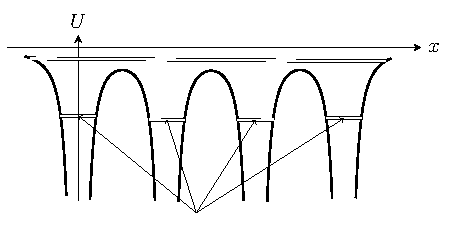
\includegraphics[width = 0.6\textwidth]{images/tikz/for_H_metall}
\end{center}
\section{О кельтском камне в форме эллипсоида}

Кельтские камни представляют собой тела, тензор инерции которых в осях симметрии системы имеет ненулевые недиагональные компоненты. Простейшим примером кельтского камня будет выступать эллипсоид вращения плотность которого постоянна со вставками двух точечных масс не изменяющих положение центра масс, но тем не менее вносящих вклад в недиагональные компоненты.

Легко убедиться (от 10 минут до получаса, если уметь брать кратные интегралы), что момент инерции однородного эллипсоида вращения с полуосями $a$, $b$, $c$ в системе в которой оси совпадают с осями симметрии системы, 0 в центре симметрии, имеет вид:
\[
	\hat{J} = 
	\begin{pmatrix}
	\frac{1}{5}m(b^2 + c^2) & 0 & 0 \\
	0 & \frac{1}{5}m(a^2 + c^2) & 0 \\
	0 & 0 & \frac{1}{5}m(a^2 + b^2) 
	\end{pmatrix}
\]
С массой $M$ добавленной в точки $(x_a, y_a, 0)$,  $(-x_a, -y_a, 0)$ мы получим следующий тензор инерции:
\[
	\hat{J} = 
	\begin{pmatrix}
	\frac{1}{5}m(b^2 + c^2) + M y_a^2 & M x_a y_a & 0 \\
	M x_a y_a & \frac{1}{5}m(a^2 + c^2) + M x_a^2 & 0 \\
	0 & 0 & \frac{1}{5}m(a^2 + b^2) 
	\end{pmatrix}
\]
В общем случае тензор инерции будет иметь вид:
\[
	\hat{J} = 
	\begin{pmatrix}
	J_{xx} & J_{xy} & J_{xz} \\
	J_{yx} & J_{yy} & J_{yz} \\
	J_{zx} & J_{zy} & J_{zz} 
	\end{pmatrix}
\]
Тело при этом пусть будет эллиптической формы, центр масс на оси симметрии системы. Тело лежит на подложке, которая действует на него моментом сил трения $\vec{M}_{fr}$ в направлении перпендикулярном подложке и противоположно компоненте угловой скорости в данном направлении. Неподвижные оси $x', y', z'$ направим как показано на рисунке. Подвижные оси будут представлять собой оси симметрии эллипсоида $x, y, z$. В подвижной системе жёстко связанной с телом на систему будут действовать силы трения (будем считать, что они приводят только к наличию момента $\vec{M}_{fr}$ в направлении перпендикулярном подложке и противоположно проекции угловой скорости на данное направление), сила реакции опоры, направленная перпендикулярно подложке $\vec{N}$, сила инерции, так как центр масс движется вообще говоря ускоренно (но она постоянна по величине и не создаёт относительно центра масс момента, в чём также легко убедиться с помощью интегрирования), центробежная сила (приводит к знаменитым эйлеровым уравнениям -- момент равен $-\vec{\omega}\times\vec{L}$), а вот сила Кориолиса равна 0, так как скорость движения точек тела в подвижной системе координат связанной с телом равна 0. Уравнения динамики вращательного движения:
\[
	\hat{J} \frac{d\vec{\omega}}{dt} + \vec{\omega}\times(\hat{J}\vec{\omega}) = \vec{N}\times\vec{R} + \vec{M}_{fr}
\]
Введём эйлеровы углы $(\psi, \theta, \phi)$. Для полного счастья нам понадобятся орты подвижной системы координат, выраженные через неподвижные. С помощью вспомогательного единичного вектора $\vec{n}$, получим:
\[
	\begin{aligned}
	& \vec{n} = \cos \psi \vec{e}_x + \sin \psi \vec{e}_y \\
	& \vec{e}'_z = \vec{e}_z \cos \theta  + \vec{n}\times\vec{e}_z \sin \theta \\
	& \vec{e}'_x = \vec{n} \cos \phi  + \vec{e}_z\times\vec{n} \sin \phi \\
	& \vec{e}'_y = \vec{e}'_z \times \vec{e}'_x = - \vec{n} \sin \phi + \vec{e}_z\times\vec{n} \cos \phi
	\end{aligned}
\]
Или в страшной форме, после долгих и утомительных преобразований:
\[
	\begin{aligned}
	& \vec{e}_x =
	[\cos \phi \cos \psi - \sin \phi \sin \psi \cos \theta] \vec{e}'_x +
	[\cos \phi \sin \psi + \sin \phi \cos \psi \cos \theta] \vec{e}'_y +
	\sin \theta \sin \phi \vec{e}_z \\
	& \vec{e}_y =
	[- \sin \phi \cos \psi - \cos \phi \sin \psi \cos \theta] \vec{e}'_x +
	[- \sin \phi \sin \psi + \cos \phi \cos \psi \cos \theta] \vec{e}'_y +
	\sin \theta \cos \phi \vec{e}_z \\
	& \vec{e}_z =
	\sin \psi \sin \theta \vec{e}'_x -
	\sin \theta \cos \psi \vec{e}'_y +
	\cos \theta \vec{e}_z \\
	\end{aligned}
\]
Отсюда просто найти и обратное преобразование, но нам потребуется всего один вектор:
\[
	\vec{e}'_z =
	\sin \theta \sin \phi \vec{e}_x -
	\sin \theta \cos \phi \vec{e}_y +
	\cos \theta \vec{e}_z
\]
Зачем он нужен? Во-первых вдоль него направлен момент сил трения, а во-вторых с его помощью можно найти нормаль к эллипсоиду, который повернули на произвольные эйлеровы углы в точке соприкосновения с подложкой и как следствие найти эту точку.
Нормаль в точке эллипсоида $(x_a, y_a, z_a)$ (ещё 10-30 минут утомительных вычислений) коллинеарна вектору:
\[
	\left\{
		\frac{x_a}{a^2},  \frac{y_a}{b^2}, \frac{z_a}{c^2}
	\right\}
\]
Поэтому:
\[
	\begin{aligned}
	& A\sin \theta \sin \phi  = \frac{x_a}{a^2} \\
	& -A\sin \theta \cos \phi  = \frac{y_a}{b^2} \\
	& A\cos \theta  = \frac{z_a}{c^2} \\
	\end{aligned}
\]
Подставляем в уравнение эллипса:
\[
	A^2[\sin^2 \theta \sin^2 \phi + \sin^2 \theta \cos^2 \phi + \cos^2 \theta] = 1
\]
\[
	A = \pm \frac{1}{\sqrt{\sin^2 \theta \sin^2 \phi + \sin^2 \theta \cos^2 \phi + \cos^2 \theta}}
\]
Знак на самом деле вполне определён, но в данный момент мне придётся долго вспоминать чему он равен. Так, так, так... Кажется $z_a$ по картинке у нас отрицательное, значит и знак отрицательный. Теперь можно чётко записать, что такое $\vec{R}$:
\[
	\vec{R} = x_a \vec{e}_x + y_a \vec{e}_y + z_a \vec{e}_z
\]
Тем самым динамические уравнения полностью определены. Кинематические уравнения я подсмотрел в одном из курсов теоретической механики:
\[
	\begin{aligned}
	& \omega_x = \dot{\psi} \sin \theta \sin \phi + \dot{\theta} \cos \phi \\
	& \omega_y = \dot{\psi} \sin \theta \cos \phi - \dot{\theta} \sin \phi \\
	& \omega_z = \dot{\psi} \cos \theta + \dot{\phi}
	\end{aligned}
\]
В таком виде для нас они бесполезны, однако вполне сойдут в виде:
\[
	\begin{aligned}
	& \dot{\psi} = \frac{\omega_x \sin \phi + \omega_y \cos \phi}{\sin \theta} \\
	& \dot{\theta} = \omega_x \cos \phi - \omega_y \sin \phi \\
	& \dot{\phi} = \omega_z - \frac{\omega_x \sin \phi + \omega_y \cos \phi}{\sin \theta} \cos \theta \\
	\end{aligned}
\]
Начальные условия для системы:
\[
	\omega_x(0) = \omega_y(0) = 0
	\quad
	\omega_z(0) = \Omega 
	\quad
	\theta(0) = \phi(0) = \psi(0) = 0 
\]
Но легко видеть, что этот случай неинтересен и ни к чему особенному приводить не должен. Более интересный случай связан с небольшими отклонениями от 0 в начальных условиях. В принципе осталось разобраться с силой реакции опоры. Из-за ускоренного движения центра масс эллипсоида она может принимать, вообще говоря значения отличные от $mg$, однако если по сравнению с $g$ добавкой можно пренебречь, то осталось перейти к моделированию. Но мне лень.
\section{$N$-мерный случай сферических координат. Якобиан. Объём гипершара, площадь гиперсферы}

Сферические координаты в $N$-мерном случае:
\[
	\begin{aligned}
	& x_1 = r \cos \theta_1 
	& x_1 \in (-\infty, \infty) \Rightarrow \theta_1 \in (0, \pi)\\
	& x_2 = r \sin \theta_1 \cos \theta_2 
	& x_2 \in (-\infty, \infty) \Rightarrow \theta_2 \in (0, \pi)\\
	& \ldots \\
	& x_{N - 1} = r \sin \theta_1 \sin \theta_2 \cdot \ldots \cdot \sin \theta_{N - 2} \cos \theta_{N-1} 
	& x_{N - 1} \in (-\infty, \infty) \Rightarrow \theta_{N - 1} \in (0, \pi)\\
	& x_{N} = r \sin \theta_1 \sin \theta_2 \cdot \ldots \cdot \sin \theta_{N - 2} \sin \theta_{N-1} 
	& \text{ НО: } x_{N} \in (-\infty, \infty) \Rightarrow \theta_{N - 1} \in (0, 2 \pi)
	\end{aligned}
\]
\[
	r > 0
\]

Якобиан:
\[
	J = 
	\frac{\partial(x_1, x_2, \ldots, x_N)}{\partial(r, \theta_1, \theta_2, \ldots, \theta_{N- 1})} =
	\begin{vmatrix}
	\cos \theta_1 & 
	- r \sin \theta_1 & 
	0 & 
	0 & 
	\ldots & 
	0 \\
	\sin \theta_1 \cos \theta_2 &
	r \cos \theta_1 \cos \theta_2 &
	- r \sin \theta_1 \sin \theta_2 &
	0 &
	\ldots &
	0 \\
	\sin \theta_1 \sin \theta_2 \cos \theta_3 &
	r \cos \theta_1 \sin \theta_2 \cos \theta_3 &
	r \sin \theta_1 \cos \theta_2 \cos \theta_3 &
	- r \sin \theta_1 \sin \theta_2 \sin \theta_3 &
	\ldots &
	0 \\
	\ldots &
	\ldots &
	\ldots &
	\ldots &
	\ldots &
	\ldots \\
	\end{vmatrix}
\]
Выносим $r$ за знак определителя, раскладываем по первой строке и выносим всё, что можно вынести за знак определителя:
\[
	\begin{gathered}
	J = r^{N - 1} J_N(\theta_1, \ldots, \theta_{N - 1}) = 
	r^{N - 1} [\cos^2 \theta_1 \sin^{N - 2} \theta_1 J_{N - 1}(\theta_2, \ldots, \theta_{N - 1}) + \sin^2 \theta_1 J_{N - 1}(\theta_2, \ldots, \theta_{N - 1})]  =  
	\\ =
	r^{N - 1} \sin^{N - 2} \theta_1 J_{N - 1}(\theta_2, \ldots, \theta_{N - 1})
	\\ =
	r^{N - 1} \sin^{N - 2} \theta_1 \sin^{N - 3} \theta_2 \cdot \ldots \cdot \sin \theta_{N - 2}
	\end{gathered}
\]

Площадь гиперсферы:
\[
	S_N = \int\limits_{\theta} r^{N - 1} \sin^{N - 2} \theta_1 \sin^{N - 3} \theta_2 \cdot \ldots \cdot \sin \theta_{N - 2} d\theta_1 \ldots d\theta_{N - 1}
\]
Воспользуемся соотношением:
\[
	\int\limits_0^\pi \sin^k x dx = \frac{\Gamma\left(\frac{k + 1}{2}\right)}{\Gamma\left(\frac{k + 2}{2}\right)} \pi^{1/2}
\]
\[
	S_N = 2 \pi r^{N - 1} \pi^{(N - 2)/2} \frac{\Gamma(1)}{\Gamma\left(\frac{N}{2}\right)} =
	\frac{2 \pi^{N/2}}{\Gamma\left(N/2\right)} r^{N - 1}
\]
Объём гипершара:
\[
	V_N = \int\limits_0^r S_N dr = \frac{2 \pi^{N/2}}{N\Gamma\left(N/2\right)} r^{N} =
	\frac{\pi^{N/2}}{\Gamma\left((N + 2)/2\right)} r^{N}
\]
\section{Энергия, передаваемая от молекулы к молекуле в одноатомном идеальном газе}

Вопрос интересен тем, что позволяет оценить насколько велика по отношению к энергии молекулы энергия передаваемая другой молекуле. Будем считать, что молекула при соударении просто переходит из одной группы молекул с энергией в данном диапазоне в другую группу с энергией в другом диапазоне. Передаваемая в этом процессе энергия будет характеризоваться величиной:
\[
	\frac{p_1'^2}{2M} - \frac{p_1^2}{2M}
\] 
Функция распределения в равновесном состоянии для идеального газа:
\[
	f(p_1, p_1') = 
	A \exp \left(
	- \frac{p_1^2 + p_1'^2}{2MkT}
	\right)	p_1^2 p_1'^2
\]
Найдём нормировочную константу:
\[
	\int\limits_0^\infty \! \int\limits_0^\infty 
	A \exp \left(
	- \frac{p_1^2 + p_1'^2}{2MkT}
	\right)	p_1^2 p_1'^2 dp_1\,dp_1'
\]
\[
	\int\limits_0^\infty e^{- \alpha p^2} p^2 dp = 
	- \frac{\partial}{\partial \alpha} \int\limits_0^\infty e^{- \alpha p^2} dp
	= - \frac{1}{2} \frac{\partial}{\partial \alpha} \sqrt{\frac{\pi}{\alpha}}
	= \frac{\sqrt{\pi}}{4\alpha^{3/2}}
\]
\[
	\int\limits_0^\infty \! \int\limits_0^\infty 
	A \exp \left(
	- \frac{p_1^2 + p_1'^2}{2MkT}
	\right)	p_1^2 p_1'^2 dp_1\,dp_1'
	=
	A \frac{8M^3k^3T^3\pi}{16} = 1
\]
\[
	A = \frac{2}{M^3k^3T^3\pi}
\]
Очевидно, что среднее значение рассматриваемой характеристики равно 0. Найдём дисперсию:
\[
	\int\limits_0^\infty \! \int\limits_0^\infty 
	A \left(\frac{p_1'^2}{2M} - \frac{p_1^2}{2M}\right)^2\exp \left(
	- \frac{p_1^2 + p_1'^2}{2MkT}
	\right)	p_1^2 p_1'^2 dp_1\,dp_1' = (*)
\]
Найдём вспомогательные интегралы:
\[
	\int\limits_0^\infty e^{- \alpha p^2} p^4 dp = 
	\frac{1}{2} \frac{\partial^2}{\partial \alpha^2} \sqrt{\frac{\pi}{\alpha}} =
	\frac{3\sqrt{\pi}}{8\alpha^{5/2}}
\]
\[
	\int\limits_0^\infty e^{- \alpha p^2} p^6 dp = 
	\frac{1}{2} \frac{\partial^3}{\partial \alpha^3} \sqrt{\frac{\pi}{\alpha}} =
	\frac{15\sqrt{\pi}}{16\alpha^{7/2}}
\]
\[
	(*) = \frac{A}{4M^2} \frac{30\sqrt{\pi}}{16\alpha^{7/2}} \frac{\sqrt{\pi}}{4\alpha^{3/2}} -
	2\frac{A}{4M^2} \frac{3\sqrt{\pi}}{8\alpha^{5/2}}\frac{3\sqrt{\pi}}{8\alpha^{5/2}}
	=
	\frac{A}{4M^2}  \frac{(15 - 9)\pi}{32\alpha^{5}} = 
	\frac{16\alpha^{3}}{4M^2\pi} \frac{3\pi}{16\alpha^{5}} =
	\frac{3}{4M^2\alpha^{2}} = 
	\frac{3M^2k^2T^2}{M^2} = 3 k^2 T^2
\]
Стандартное отклонение:
\[
	\sigma = \sqrt{3} kT
\]
Данная величина превосходит среднее значение энергии отдельной молекулы одноатомного идеального газа!
\section{Странные вещи}

\subsection{Тождество для д...а}

\[
	f(x)\delta(x - x_0) + [F(x) - F(x_0)] \delta'(x - x_0) = 0, \qquad F(x) = \int f(x) dx
\]

\textit{Док-во:}

Продифференцируем тождество:
\[
	F(x) \delta(x - x_0) = F(x_0) \delta(x - x_0)
\]
Просто, не правда ли? В чём подвох? При представлении $\delta$-функции в форме гауссовского предела доказательство упирается в весьма необычные трудности. В частности требуется доказать следующее равенство:
\[
	\lim\limits_{a \to 0} \frac{1}{a}\left(1 - 2 \frac{(x - x_0)^2}{a^2}\right) e^{- \cfrac{(x - x_0)^2}{a^2}} = \lim\limits_{a \to 0} \frac{1}{a} e^{- \cfrac{(x - x_0)^2}{a^2}}
\]
И вот вопрос: как это сделать строго? Казалось бы, что сложного, рассмотрим два случая $x = x_0$ и $x \ne x_0$, равенство выполняется? - Да! Но мне это доказательство не даёт покоя. Кажется, что я что-то упускаю. Тем более, что из тождества следует:
\[
	\delta'(x -x_0) = \frac{1}{x_0 - x} \delta(x -x_0)
\]

\subsection{Ещё одно странное тождество}

\[
	(f(x) \eta(x - a))''_{xx} = f''(x) \eta(x - a) + f'(a) \delta(x - a) + f(a) \delta'(x - a)
\]

\textit{Док-во:}

Снова всё тривиально:
\[
	(f(x) \eta(x - a))''_{xx} = (f'(x) \eta(x - a) + f'(x) \delta(x - a))'_x = (f'(x) \eta(x - a) + f'(a) \delta(x - a))'_x =
	f''(x) \eta(x - a) + f'(a) \delta(x - a) + f(a) \delta'(x - a)
\]

\subsection{Функция отличная от нуля в одной единственной точке}

\[
	f(x) = 2A\eta(-|x-a|) = \begin{cases}
	A, & x = a\\
	0, & x\ne a
	\end{cases}
\]
Наибольший интерес представляет её производная:
\[
	f'(x) = -2A\delta(-|x-a|)\sign(x -a) = 0
\]
Не правда ли замечательно! Теперь решение уравнения:
\[
	y' = 0,\qquad y(0) = y_0
\]
будет выглядеть так:
\[
	y = y_0+\sum\limits_{i, a_i \ne 0} 2 C_i \eta(-|x-a_i|)
\]
То есть в классе функций с разрывами решений бесконечно много! 

Как мне подсказал Antony я вообще говоря не прав, так как здесь имеет место неопределённость вида $\infty\times 0$. Представление в форме предела последовательности для $\delta-$функции, приводит тем не менее к результатам изложенным выше, но при одном дополнительном условии, что пределы можно менять местами, что скорее всего также неправильно. Ещё один способ мог бы быть связан с представлением решения в форме предела:
\[
	\lim\limits_{b \to 0} \eta(x - a - b) - \eta(x - a)
\]
Но как следует из определения $\eta-$функции это тождественно 0. И вопрос о правильности полученных результатов остаётся открытым. Вдогонку к данной проблеме можно рассмотреть следующее интересное тождество:
\[
	\sign^2(x) = |\sign(x)|
\]
Продифференцируем его:
\[
	4 \sign(x) \delta(x) = \sign(\sign(x)) 2\delta(x) = 2 \sign(x) \delta(x) 
\]
Если бы можно было сократить всё лишнее было бы:
\[
	4 = 2
\]
Но к счастью сократить ничего нельзя. Однако, отсюда следует:
\[
	 2 \sign(x) \delta(x) = 0
\]

\subsection{Функция для вычисления площади пересечения треугольника с полуплоскостью}

Рассмотрим треугольник, один из катетов, которого лежит на оси абсцисс, другой параллелен оси ординат и прямую, параллельную оси ординат, делящую плоскость на две полуплоскости, как показано на рисунке:
\begin{center}
	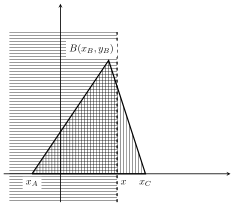
\includegraphics{images/png/triangle_func.png}
	%\usetikzlibrary{patterns}
\begin{tikzpicture}

\draw[thick,-stealth]  (0,-1) -- (0,6);
\draw[thick,-stealth] (-2,0) -- (6,0);
\draw[very thick, pattern=vertical lines] (-1,0) -- (1.7, 4) -- (3,0) -- (-1, 0);
\draw[very thick, dashed] (2, -1) -- (2, 5);
\path[pattern=horizontal lines] (2, -1) rectangle (-1.8, 5);

\node[below, fill = white] at (-1,-0.1) {$x_A$};
\node[above, fill = white] at (1.1,4.1) {$B(x_B, y_B)$};
\node[below] at (3,-0.1) {$x_C$};
\node[below right] at (2,-0.1) {$x$};

\end{tikzpicture}
\end{center}
Площадь области с двойной штриховкой:
\[
	S_+(x, x_A, x_B, x_C, y_B) = 
	\begin{cases}
	0, & x < x_A; \\
	\frac{1}{2} y_B \frac{(x - x_A)^2}{x_B - x_A}, & x_A < x < x_B; \\
	\frac{1}{2} y_B \left[(x_B - x_A) + \frac{2 x_C - x - x_B}{x_C - x_B} (x - x_B)\right] , & x_B < x < x_C; \\
	\frac{1}{2} y_B (x_C - x_A), & x_C < x.
	\end{cases}
\]
Другая полуплоскость, даёт область с одинарной штриховкой:
\[
S_-(x, x_A, x_B, x_C, y_B) = 
\begin{cases}
\frac{1}{2} y_B (x_C - x_A), & x < x_A; \\
\frac{1}{2} y_B \left[(x_C - x_B) + \frac{x_B + x - 2 x_A}{x_B - x_A} (x_B - x)\right], & x_A < x < x_B; \\
\frac{1}{2} y_B \frac{(x_C - x)^2}{x_C - x_B} , & x_B < x < x_C; \\
0, & x_C < x.
\end{cases}
\]
Первую из этих функций можно представить в виде:
\[
	\begin{aligned}
	& S_+(x, x_A, x_B, x_C, y_B) =  
	\frac{1}{2} y_B \frac{(x - x_A)^2}{x_B - x_A} \eta(x - x_A) \eta(x_B - x)  + \\ & +
	\frac{1}{2} y_B \left[(x_B - x_A) + \frac{2 x_C - x - x_B}{x_C - x_B} (x - x_B)\right] \eta(x - x_B) \eta(x_C - x) +
	\frac{1}{2} y_B (x_C - x_A) \eta(x - x_C)
	\end{aligned}
\]
Здесь следует отметить, что представление возможно только если $x_A < x_B < x_C$. Именно для этого случая записаны все выражения выше.
\section{Весёлые интегралы}
Произвольные постоянные в неопределённых интегралах далее опущены.
\begin{enumerate}
	\item 
	\[
		\int \frac{dx}{\sqrt{x^2 + 1}} = \mathrm{arsh\,}x = \ln |x + \sqrt{x^2 + 1}|
	\]
	\item
	\[
		\int \sqrt{x^2 + 1} dx = 
		x \sqrt{x^2 + 1} - \int \frac{x^2}{\sqrt{x^2 + 1}}dx =
		x \sqrt{x^2 + 1} - \int \sqrt{x^2 + 1}dx + \int \frac{dx}{\sqrt{x^2 + 1}}
	\]
	\[
		\Rightarrow \quad
		\int \sqrt{x^2 + 1} dx = \frac{x \sqrt{x^2 + 1} + \ln |x + \sqrt{x^2 + 1}|}{2}
	\]
	\item
	\[
		\int \frac{\sqrt{x}}{\sqrt{x-1}} dx = 
		\int 2 \sqrt{x} d\sqrt{x-1} =
		[\sqrt{x - 1} = p]
		= 2 \int \sqrt{p^2 + 1} dp = 
		\sqrt{x} \sqrt{x-1}+ \ln |\sqrt{x - 1} + \sqrt{x}|
	\]
	\item
	\[
		\int \frac{x\,dx}{\sqrt{px^2 - ax - b}} = 
		\frac{1}{\sqrt{p}} \int \frac{\Big(x - \cfrac{a}{2p} + \cfrac{a}{2p}\Big)\,dx}{\sqrt{\Big(x - \cfrac{a}{2p}\Big)^2 - \Big(\cfrac{a^2}{4p^2} + \cfrac{b}{p}\Big)}}
		= \frac{1}{\sqrt{p}} \sqrt{\Big(x - \cfrac{a}{2p}\Big)^2 - \Big(\cfrac{a^2}{4p^2} + \cfrac{b}{p}\Big)} + 
		\frac{1}{\sqrt{p}} \cfrac{a}{2p} \,\mathrm{arch\,} \frac{x - \cfrac{a}{2p}}{\sqrt{\cfrac{a^2}{4p^2} + \cfrac{b}{p}}}
	\]
	\item
	\[
		\int\limits_a^b |x| dx = 
		\begin{cases}
		\frac{b^2 - a^2}{2}, & 0 < a < b \\
		\frac{a^2 + b^2}{2}, & a < 0 < b \\
		\frac{a^2 - b^2}{2}, & a < b < 0
		\end{cases}
		=
		\frac{\sign(b) b^2 - \sign(a) a^2}{2}
	\]
	\[
		\int |x| dx = \int x \sign (x) dx = \sign (x) \frac{x^2}{2}
	\]
	\[
		\int x^n \sign (x) dx = \sign (x) \frac{x^{n+1}}{n + 1}
	\]
	\item
	\[
		\int\limits_{-\infty}^\infty\int\limits_{-\infty}^\infty e^{-x^2 - y^2} dx dy =
		2\pi \int\limits_0^\infty r e^{-r^2} dr = - \pi e^{-r^2} \Big|_0^\infty = \pi 	
	\]
	\[
		\int\limits_{-\infty}^{\infty} e^{-x^2} dx = \sqrt{\pi}
	\]
	\item 
	\[
		\Gamma(s) = \int\limits_0^\infty x^{s - 1} e^{-x} dx = 
		-x^{s-1} e^{-x} \Big|_0^\infty + (s - 1) \int\limits_0^\infty x^{s - 2} e^{-x} dx = (s - 1) \Gamma (s - 1)
	\]
	\[
		\Gamma(n) = (n - 1)!
	\]
	\[
		\Gamma(1/2) = \int\limits_0^\infty x^{-1/2} e^{-x} dx = 2 \int\limits_0^\infty e^{-x} dx^{1/2} =
		2 \int\limits_0^\infty e^{-t^2} dt = \int\limits_{-\infty}^\infty e^{-t^2} dt = \sqrt{\pi}
	\]
	\[
		\Gamma((n + 1)/2) = \frac{(n - 1)(n - 3)...(n - 2p - 1)}{2^{p+1}} \Gamma((n - 2p - 1)/2) =
		\begin{cases}
		\frac{(n - 1)!!}{2^{n/2}} \sqrt{\pi} & \text{$n$ -- чётное} \\
		\frac{(n - 1)!!}{2^{(n - 1)/2}} & \text{$n$ -- нечётное}
		\end{cases} 
	\]
	\[
		\frac{\Gamma\left(\frac{n + 1}{2}\right)}{\Gamma\left(\frac{n}{2}\right)}
		=
		\begin{cases}
		\frac{(n - 1)!! 2^{(n - 2)/2}}{(n - 2)!! 2^{n/2}} \sqrt{\pi} & \text{$n$ -- чётное} \\
		\frac{(n - 1)!! 2^{(n - 1)/2}}{(n - 2)!! 2^{(n - 1)/2}} \frac{1}{\sqrt{\pi}} & \text{$n$ -- нечётное}
		\end{cases}
		=
		\begin{cases}
		\frac{(n - 1)!!}{(n - 2)!!} \frac{\sqrt{\pi}}{2} & \text{$n$ -- чётное} \\
		\frac{(n - 1)!!}{(n - 2)!!} \frac{1}{\sqrt{\pi}} & \text{$n$ -- нечётное}
		\end{cases}
	\]
	\[
		\frac{\Gamma\left(\frac{n + 1}{2}\right)}{\Gamma\left(\frac{n + 2}{2}\right)}
		=
		\begin{cases}
		\frac{(n - 1)!!}{n!!} \sqrt{\pi} & \text{$n$ -- чётное} \\
		\frac{(n - 1)!!}{n!!} \frac{2}{\sqrt{\pi}} & \text{$n$ -- нечётное}
		\end{cases}
	\]
	\item
	\[
		I_n = \int\limits_0^\pi \sin^n x \, dx = - \cos x \sin^{n - 1} x \Big|_0^\pi + (n - 1) \int\limits_0^\pi \sin^{n - 2} x \cos^2 x \, dx = 
		(n - 1) I_{n - 2} - (n - 1) I_n 
	\] 
	\[
		I_n = \frac{n - 1}{n} I_{n - 2} = \frac{(n - 1)(n - 3)...(n - 2p +  1)}{n(n - 2)...(n - 2p + 2)} I_{n - 2p} =
		\begin{cases}
		\frac{(n - 1)!!}{n!!} \pi  & \text{$n$ -- чётное}\\
		\frac{(n - 1)!!}{n!!} 2 & \text{$n$ -- нечётное}
		\end{cases}
		=
		\frac{\Gamma\left(\frac{n + 1}{2}\right)}{\Gamma\left(\frac{n + 2}{2}\right)} \sqrt{\pi}
	\]
	\item
	\[
		\delta(x) = \frac{1}{2\pi} \int\limits_{-\infty}^{\infty} e^{ikx} dk = \frac{1}{\pi} \int\limits_{0}^{\infty} \cos (kx) dk
	\]
	\[
		\int\limits_{0}^{\infty} \cos (kx) dk = \pi \delta(x)
	\]
	\[
		\int\limits_{0}^{\infty} \sin (kx) dk = [kx = k'x + \pi/2] = \int\limits_{-\frac{\pi}{2x}}^{\infty} \cos (k'x) dk' =
		\pi \delta(x) - \int\limits_{-\frac{\pi}{2x}}^{0} \cos (k'x) dk' = 
		\pi \delta(x) - \frac{\sin (k'x)}{x} \Big|_{-\frac{\pi}{2x}}^0 = 
		\pi \delta(x) - \frac{1}{x}
	\]
	\item 
	\[
		\pi \delta^{(2n+1)}(x) = (-1)^{n + 1} \int\limits_{0}^{\infty} k^{2n + 1} \sin (kx) dk
	\]
	\[
		\pi \delta^{(2n)}(x) - (2n)! \frac{1}{x^{2n+1}} = (-1)^{n} \int\limits_{0}^{\infty} k^{2n} \sin (kx) dk
	\]
	\[
		\int\limits_{0}^{\infty} k^{2n + 1} \sin (kx) dk = (-1)^{n + 1} \pi \delta^{(2n+1)}(x)
	\]
	\[
		\int\limits_{0}^{\infty} k^{2n} \sin (kx) dk = (-1)^{n} \pi \delta^{(2n)}(x) - (-1)^{n} (2n)! \frac{1}{x^{2n+1}}
	\]
	\[
		\int\limits_0^\infty e^{ikx} dk = \pi (1 + i) \delta(x) - \frac{i}{x}
	\]
	\[
		\int\limits_0^\infty k^n e^{ikx} dk = \pi \frac{(1 + i)}{i^n} \delta^{(n)}(x) - \frac{i(-1)^n}{i^n} \frac{n!}{x^{n+1}} =
		\pi (1 + i) (-i)^n \delta^{(n)}(x) - i^{n+1} \frac{n!}{x^{n+1}}
	\]
	\item
	\[
		\begin{gathered}
		I_n(\alpha) = \int\limits_0^\pi e^{i\alpha \cos \theta} \sin^n \theta \, d\theta = - \frac{1}{i\alpha} \int\limits_0^\pi  \sin^{n - 1} \theta \, de^{i\alpha \cos \theta} 
		=
		\frac{n - 1}{i\alpha} \int\limits_0^\pi  \sin^{n - 2} \theta \cos \theta \, e^{i\alpha \cos \theta} d\theta
		= \\ =
		- \frac{n - 1}{\alpha} \frac{\partial}{\partial \alpha} \int\limits_0^\pi  \sin^{n - 2} \theta \, e^{i\alpha \cos \theta} d\theta
		=
		- \frac{n - 1}{\alpha} \frac{\partial I_{n - 2}}{\partial \alpha} 
		=
		(-1)^k (n - 1)(n - 3)(n - 5)\cdot\ldots\cdot(n - (2k - 1)) \left(\frac{1}{\alpha} \frac{\partial}{\partial \alpha} \right)^k I_{n - 2k}
		= \\ =
		\begin{cases}
			(-1)^k (2k)!! \left(\dfrac{1}{\alpha} \dfrac{\partial}{\partial \alpha} \right)^k I_{1} & n = 2k + 1 \\
			(-1)^k (2k - 1)!! \left(\dfrac{1}{\alpha} \dfrac{\partial}{\partial \alpha} \right)^k I_{0} & n = 2k
		\end{cases}
		\end{gathered}
	\]
	\[
		\begin{gathered}
		I_1(\alpha) =
		\int\limits_0^\pi e^{i\alpha \cos \theta} \sin \theta \, d\theta
		=
		\int\limits_0^\pi 
		\left(
			J_0(\alpha) + 2\sum_{p = 1}^{\infty} i^p J_p(\alpha) \cos (p\theta) 
		\right)\sin \theta \, d\theta
		= \\ =
		\int\limits_0^\pi 
		\left(
			J_0(\alpha) \sin \theta + \sum_{p = 1}^{\infty} i^p J_p(\alpha) [\sin ((p + 1)\theta) - \sin ((p - 1) \theta)]
		\right)\, d\theta
		=
		2 J_0(\alpha) + \sum_{p = 1}^{\infty} i^p J_p(\alpha) \left[\frac{1 - (-1)^{p + 1}}{p + 1} - \frac{1 - (-1)^{p - 1}}{p - 1}\right]
		= \\ =
		2 J_0(\alpha) - 4 \sum_{p = 1}^{\infty} (-1)^p J_{2p}(\alpha) \frac{1}{4 p^2 - 1}
		= 
		-\frac{e^{i\alpha \cos \theta}}{i\alpha} \Bigg|_0^\pi = \frac{2 \sin \alpha}{\alpha}
		\end{gathered}
	\]
	\[
		I_0 (\alpha) = \int\limits_0^\pi e^{i\alpha \cos \theta} d\theta = \pi J_0(\alpha)
	\]
	Удивительно, но факт -- результат приводится к общему виду. Воспользуемся соотношениями:
	\[
		J_{k + 1/2} (\alpha) = \frac{(-1)^k \alpha^{k + 1/2}}{\sqrt{2\pi}} \left(\dfrac{1}{\alpha} \dfrac{\partial}{\partial \alpha} \right)^k \dfrac{2 \sin \alpha}{\alpha}
		\qquad
		J_{k} (\alpha) = (-1)^k \alpha^k \left(\dfrac{1}{\alpha} \dfrac{\partial}{\partial \alpha} \right)^k J_0(\alpha)
	\]
	\[
		\Gamma \left(\dfrac{n + 1}{2}\right) = 
		\begin{cases}
		\dfrac{(2k - 1)!!}{2^k} \sqrt{\pi} & n = 2k \\
		\dfrac{(2k)!!}{2^k} & n = 2k + 1
		\end{cases}
	\]
	Получаем:
	\[
		I_n(\alpha) = 
		\begin{cases}
		\Gamma \left(\dfrac{n + 1}{2}\right) 2^{k} \frac{\sqrt{2\pi}}{\alpha^{n/2}} J_{k + 1/2} (\alpha) & n = 2k + 1 \\
		\Gamma \left(\dfrac{n + 1}{2}\right) 2^{k} \frac{\sqrt{\pi}}{\alpha^{n/2}}  J_{k} (\alpha)  & n = 2k
		\end{cases}
		=
		\Gamma \left(\dfrac{n + 1}{2}\right) 2^{n/2} \sqrt{\pi} \frac{J_{n/2} (\alpha)}{\alpha^{n/2}}  
	\]
\end{enumerate}
\section{Весёлые интегралы в комплексной плоскости}

\begin{center}
\begin{longtable}{|p{0.03\textwidth}|p{0.3\textwidth}|p{0.6\textwidth}|}
	\hline
	\endfirsthead
	\hline
	\endhead
	\endfoot
	
	\hline
	\endlastfoot
	
	1 
	&
	
	$f(z)$ ограничена по модулю:
	\[
	|f(z)| < M
	\]
	
	\centering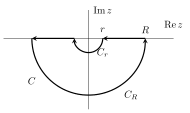
\includegraphics[width = 0.3 \textwidth]{images/png/countour_int1.png}
	&
	\[
	\begin{gathered}
	\oint\limits_C \frac{e^{-ia z}}{z} f(z) dz = 
	\int\limits_{C_R} + \int\limits_{R}^{r} + \int\limits_{C_r} + \int\limits_{-r}^{-R}
	\end{gathered}
	\]
	\[
	\begin{gathered}
	\left|
	\int\limits_{C_R} \frac{e^{-ia z}}{z} f(z) dz 
	\right| 
	= \left| 
	\int\limits_{\pi}^{2\pi} i e^{-ia R e^{i\varphi}} f(R e^{i\varphi}) d\varphi
	\right|
	\leqslant 
	\int\limits_{\pi}^{2\pi} e^{a R \sin \varphi} M d \varphi = \\ =
	M e^{a R \sin \varphi^*} \pi\Big|_{\varphi^* \in (\pi, 2\pi)} \underset{R \to \infty}{\to} 0
	\end{gathered}
	\]
	\[
	\begin{gathered}
	\lim\limits_{r \to 0} \int\limits_{C_r} \frac{e^{-ia z}}{z} f(z) dz =
	\lim\limits_{r \to 0} \int\limits_{2\pi}^{\pi} i e^{-ia R e^{i\varphi}} f(r e^{i\varphi}) d\varphi =
	- i f(0) \pi
	\end{gathered}
	\]
	\[
	\begin{gathered}
	\fint\limits_{-\infty}^{\infty} \frac{e^{-ia z}}{z} f(z) dz =
	- i f(0) \pi
	\end{gathered}
	\]
	Можно показать, что при изменении знака $a$ изменится контур (будет вверху), направление обхода и как следствие знак результата.
	\[
	\begin{gathered}
	\fint\limits_{-\infty}^{\infty} \frac{e^{ia z}}{z} f(z) dz =
	i f(0) \pi \sign a
	\end{gathered}
	\]
	Отсюда можно получить более общее выражение:
	\[
	\begin{gathered}
	\fint\limits_{-\infty}^{\infty} \frac{e^{ia z}}{z - z_0} f(z) dz =
	i e^{iaz_0} f(z_0) \pi \sign a
	\end{gathered}
	\]
	\\ 
\end{longtable}
\end{center}
\section{Весёлые диффуры}

\begin{enumerate}
	\item
		\[
			\begin{aligned}
				& g'' = \frac{a}{2g^2} + \frac{b}{g^3} \\
				& \Rightarrow g'^2 = g'^2_0 + \frac{a}{g_0} + \frac{b}{g^2_0} - \frac{a}{g} - \frac{b}{g^2} =
				p - \frac{a}{g} - \frac{b}{g^2} \\
				& \int\limits_{g_0}^{g} \frac{g\,dg}{\sqrt{pg^2 - ag - b}} = t - t_0
			\end{aligned}
		\]
\end{enumerate}

\end{document}